\status{started}
\chapter{Introduction}

\begin{refsection}

{\itshape
Here we will provide an overview of the following chapters as well as define the theoretical and experimental background for this work. 
The first section will be dedicated to the outline of this thesis, to aid the readers. 
A somewhat shallow review of the particle physics searches at PSI will follow, with some in-depth dive into the subjects which are close to the core of this thesis. 
This will be complemented by the description of the different facilities at PSI, with a final section dedicated to the Proton Ionization Facility.\\ 
This whole chapter relies heavily on references \textcite{Signorelli} \cite{PSI:review:2021}.}

\status{started}
\section{Outline of this thesis}
    The structure of this Thesis might differ slightly from the norm. 
    While most of my colleagues dedicated their work to a singular subject, like a particular detector or theory, my effort during the course of this Ph.D. has been spread on a wider angle.
    At first glance, this work might seem the result of three separate projects, namely MEG, MuEDM, and muCool. 
    In fact, the spirit in which this Thesis has been developed is orthogonal to the chapters themselves: the overall progress of muonic particle physics experiments.

    \begin{outline}
        \1 Introduction: theory, PSI facilities and key experiments
        \1 muCool (?)
        \1 muEDM: introduction, entrance detector, tracker
        \1 MEG: introduction and CW, Liquid Hydrogen target, X17 search
    \end{outline}

\status{review}
\section{Particle physics at Paul Scherrer Institute} 
    Belonging to ETH domain and formed in 1988 as a national laboratory, the Paul Scherrer Institute (PSI) is the largest federal research institute in Switzerland. 
    PSI hosts the world's most powerful proton accelerators, with an average power of \SI{1.4}{MW} and a beam current of over \SI{2}{mA}.
    On top of the proton facility, in the last 10 years, a neutron spallation target has been added for ultracold neutrons production.  
    PSI is renowned for its extensive research across a wide range of scientific disciplines.
    With its world-class facilities and expertise, PSI plays a pivotal role in advancing our understanding of fundamental particles and their interactions, solidifying its position as a key player in the field of particle physics on a global scale.
    Everything discussed in this thesis is a product of the fertile environment at this Institute and the active collaborations with universities and institutions, such as INFN, around the world.
    
\status{review}
\section{Bite-size theory}
    The aim of this section is to define the framework in which (part) of particle physics research is moving. In particular, we will be focusing on the aspects which are relevant to the three experiments core of this thesis.
    The searches \gls{bsm} proceed in two main directions: \textit{intensity frontier} is used to describe the test of contributions that are too small to be experimentally accessible observing large numbers of events;
    \textit{precision frontier} is used when improving the accuracy of a specific parameter to test the agreement with the \gls{sm}.
    Searches for \gls{clfv} or neutron \gls{edm} are examples of the former type while precision \gls{qed} tests with muonium are of the latter.

    \status{review}
    \subsection{Standard Model at low energies}
        In the low energy regime \gls{qed} and \gls{qcd} are essentially `frozen', and the \gls{sm} reduces to the standard Lagrangian
        \begin{equation}
            \mathcal{L}_{QED+QCD}=\sum_{f}\bar{f}(i\cancel{D}-m_f)f-\frac{1}{4}F_{\alpha\beta}F^{\alpha\beta}-\frac{1}{4}G_{\alpha\beta}G^{\alpha\beta}
            \label{eq:sm}
        \end{equation}
        where $F$ and $G$ are the electromagnetic and gluonic field-strength tensors. The sum here is on fermions of mass $m_f$, charge $eQ_f$, and color $g_st^a_f$. For a lepton, this would mean $Q_\ell=-1$ and $t^a_\ell=0$ while for a quark $Q_q=2/3$ or $-1/3$ and $t^a_q=\lambda^a/2$, with $\lambda$ Gell-Mann matrices.
        To compute the matrix element between two lepton states we find:
        \begin{equation}
            \matrixel{\ell(p_2)}{J^a_{em}}{\ell(p_1)} =\bar{u}(p_2,m_\ell)\left(F^{(\ell)}_1(q^2)\gamma^a+F^{(\ell)}_2(q^2)\frac{i\sigma^{\alpha\beta}q_\beta}{2m_\ell} \right)u(p_1,m_\ell)
            \label{eq:matrix}
        \end{equation}
        Here $u$ and $\bar{u}$ are the spinors and the two states are with momenta $p_1$ and $p_2=p_1+q$ while $F_1^{(\ell)}$ and $F_1^{(\ell)}$ are related respectively to the electric charge and the \gls{amm}. 
        In particular, fort the \gls{amm} we find  
        \begin{equation}
            F_2^{(\ell)}(0) = a_\ell = \frac{(g-2)_\ell}{2}  
            \label{eq:amm}
        \end{equation}
        Even when considering non point-like particles, like nucleons $N\in \{p,n\}$ the form used in \ref{eq:matrix} holds and we find:
        \begin{equation}
            \matrixel{N(p_2)}{J^a_{em}}{N(p_1)} =\bar{u}(p_2,m_N)\left(F^{(N)}_1(Q^2)\gamma^a+F^{(N)}_2(Q^2)\frac{i\sigma^{\alpha\beta}q_\beta}{2m_N} \right)u(p_1,m_N)
        \end{equation}
        Here $Q^2\equiv -q^2$ and, while \ref{eq:amm} holds, $F_2^{(N)}$ depends on strong dynamics.
        In the case of nucleons, it is often useful to introduce the \textit{electric} and \textit{magnetic form factors}
        \begin{equation*}
            G^{(N)}_E(Q^2)\equiv F_1^{(N)}(Q^2)-\frac{Q^2}{4m_N^2}F_2^{(N)}(Q^2);
            \quad 
            G^{(N)}_M(Q^2)\equiv F_1^{(N)}(Q^2)+F_2^{(N)}(Q^2)
        \end{equation*}
        It is of particular interest that, in the limit for small $Q^2$, the form factors can be understood as Fourier transform of extended classical `charge' distributions $\rho_i(r)$
        \begin{equation*}
            F_i(Q^2) = \int \dd[3]\bm{r}e^{-i\bm{q\cdot r}}\rho_i(r) = \int \dd[3]\bm{r}\rho_i(r) +\frac{1}{6}Q^2 \int \dd[3]\bm{r}r^2\rho_i(r)  + \dots
        \end{equation*}
        From this, we can write the general expression for the second moment of the charge distribution or \gls{edm}. This relation is used for example when determining the charge and magnetic radii of the proton. 
        \begin{equation}
            r^2_i\equiv\frac{1}{N}\int \dd[3]\bm{r}r^2\rho_i(r) = -6\frac{1}{N}\evaluated{\frac{dF_i(Q^2)}{dQ^2}}_{Q^2=0};
            \quad
            N=
            \begin{cases}
                1 & \text{if}\ F_i(0)=0,\\
                F_i(0) &\text{else}.
            \end{cases}
        \end{equation}
        When introducing the weak interaction we arrange fermions in \textit{left-handed doublets} and \textit{right-handed singlets}.
        We then define the \textit{charged weak current} $J_{cc}^\alpha$, a similar \textit{neutral weak current} $J_{cn}^\alpha$ and we find
        \begin{equation}
            \mathcal{L}_{EW}=eA_\alpha J_{em}^\alpha + \frac{g}{\sqrt{2}}\left(W^+_\alpha J_{cc}^\alpha+\text{h.c.} \right) + g_zZ_\alpha J^\alpha_{nc};
            \quad
            J^\alpha_{cc}=\sum_\ell \bar{\nu}_\ell\gamma^\alpha P_L\ell+\sum_{ij}V_{ij}\bar{u}_i\gamma^\alpha P_L d_j
        \end{equation}
        where $g=e/\sin{\vartheta_W}$, $g_Z=e/\cos{\vartheta_W}$ are the $SU(2)_L$ coupling  expressed trough the Weinberg mixing angle $\vartheta_W$. Only the left-handed fermions are coupled (through $P_L\equiv (1-\gamma_5)/2$) and, in the sum over the quark, the \gls{ckm} matrix $V_{ij}$ describes the flavor-changing effect.
        When dealing with masses much smaller than $m_W$ and $m_Z$ the result is the `effective' Fermi theory current-current interaction
        \begin{equation}
            \mathcal{L}_{4F}= -\frac{4 G_F}{\sqrt{2}} \left( J_{cc}^\alpha(J_{cc})^\dag_\alpha + J^\alpha_{nc}(J^\alpha_{nc})_\alpha\right)
        \end{equation}
        In this equation $4G_F/\sqrt{2}=g^2/(2m_W^2)$ and using the definitions for $J_{nc/cc}^\alpha$ we end up with the vector contact interactions.
        In this framework photons and gluons are the only gauge bosons and the gauge symmetry of the \gls{sm} $SU(3)_c\times SU(2)_L\times U(1)_Y$ is reduced to \gls{qcd} and \gls{qed}: $SU(3)_c\times U(1)_{em}$.
        We can write a 6-dimension vector operator which links 4 fermions in a generic form
        \begin{equation}
            [O^{XY}_{f}]_{ijkl}=(\bar{\psi}_i\gamma^\alpha P_X \psi_j)(\bar{\psi}_k\gamma_\alpha P_Y \psi_l)
        \end{equation}
        where $X,Y \in {L,R}$ and ${i,j,k,l}$ are generation indices. There are many such operators because $\psi$ could be leptons or quarks but the integration of the $W$ and $Z$ generates only a subset (i.g. we have no \gls{clfv} operator due to accidental symmetries).
        In a similar fashion, an operator will be a 6-dimension scalar when removing the $\gamma$ matrices or a 5-dimension dipole operator including photons and gluons:
        \begin{equation}
            [O^D_{f\gamma}]_{ij}=(\bar{\psi}_i\sigma_{\alpha\beta}P_R\psi_j)F^{\alpha\beta};
            \quad
            [O^D_{qG}]_{ij}=(\bar{\psi}_i\sigma_{\alpha\beta}G^{\alpha\beta}P_R\psi_j)
        \end{equation}
        
    \status{review}
    \subsection{Beyond Standard Model at low-energy}
        There is no shortage of \gls{bsm} models and one way of (roughly) classifying them would be by the masses and coupling strengths of the particles they introduce. 
        Light \gls{bsm} particles have small couplings to \gls{sm} particles, which would explain the small contribution to physical observables. Prominent examples are dark photons, axions and \gls{alp}.
        Axions in particular were proposed as a solution to the small value of the \gls{cp} violating \gls{qcd} $\vartheta$ parameter.
        When discussing Heavy \gls{bsm} particles we can follow the process of `integration' shown for $W$ and $Z$ in this section, in an \gls{eft} approach.
        As long as the \gls{bsm} physics respects \gls{qed} and \gls{qcd} gauge symmetry and involves `large' mass scale $\Lambda$ ($m_b<\lambda<m_W$), it can be integrated out. 
        This way we add higher-dimensional operators to the \gls{sm} Lagrangian, obtaining a \gls{left}
        \begin{equation}
            \mathcal{L}_{LEFT}= \mathcal{L}_{QED+QCD}+\frac{1}{\Lambda}\sum_iC^{(5)}_iO^{(5)}_i +\frac{1}{\Lambda^2}\sum_iC^{(6)}_iO^{(6)}_i +\dots
                \label{eq:left}
        \end{equation}
        To parameterize low-energy observables and measuring (or constraining) associated parameters is not an easy task: a prime example would be the Michel decay (which we will discuss in the following sections), generalized in terms of scalar vector and tensor contact interactions or the similar effort for the \gls{clfv} $\mu\rightarrow e \gamma$ and $\mu \rightarrow eee$ withe lepton-flavor-violating contact interactions.
        If the \gls{bsm} physics appears at a scale larger than $m_W$, we first have to develop a \gls{smeft}.
        The details on how this is achieved are outside our purpose but, including all the different gauge fields, Higgs doublet, left-handed doublets, and right-handed singlet (respecting the $SU(3)_c\times SU(2)_L\times U(1)_Y$ gauge symmetry) we find
        \begin{equation}
            \mathcal{L}_{SMEFT}=\mathcal{L}_{SM}+\frac{1}{\Lambda}(C^{(5)}O^{(5)}+\text{h.c.}) +\frac{1}{\Lambda^2}\sum_iC^{(6)}_iO^{(6)}_i +\dots
            \label{eq:smeft}
        \end{equation}
        We can now re-evaluate the matrix in \ref{eq:matrix} element using \ref{eq:smeft} instead of \ref{eq:sm}.
        We will leave the details of the calculation under the hood but the result we get is the following
        \begin{equation}
        \begin{split}
            \matrixel{f(p_2)}{J^\alpha_{em}}{f(p_1)} = 
            \bar{u}(p_2,m_f) \left(F^{(f)}_1(q^2)\gamma^a+ \left(F^{(f)}_2(q^2)- i\gamma_5F^{(f)}_3(q^2)\right) \frac{i\sigma^{\alpha\beta}q_\beta}{2m_f}+ \right.\\
            \left. F^{(f)}_4(q^2)\frac{1}{m_f^2}(q^2\gamma^\alpha-2m_fq^\alpha)\gamma_5 \right) u(p_1,m_f)
        \end{split}
        \end{equation}
        It is of interest that the \gls{cp}-violating $F_3$ form factor is linked to the \gls{edm} of the lepton $d_f$
        \begin{equation}
            d_f=\frac{eF_3^{(f)}(0)}{2m_f}
            \label{eq:edm}
        \end{equation}
        In the \gls{sm}, $d_f$ receives contributions from quarks at 3-loops and leptons at 4-loops (induced by \gls{cp}-violation in the \gls{ckm}). 
        When considering protons and neutrons there is an additional contribution from the \gls{cp} violating \gls{qcd} $\vartheta$ parameter (found to be extremely low constraining the neutron \gls{edm}).
        For completeness sake, $J_{cc}^\alpha$ give rise to matrix elements between different $SU(2)$ doublets, like $(\nu_\ell,\ell)$ or $(p,n)$. This leads to muon and beta decay or quasi-elastic scattering $\ell p\rightarrow \nu_\ell n$.

    \status{review}
    \subsection{Muon}
        The muon is the lepton with the intermediate mass of $m_\mu \approx 105.66$ MeV and it is unstable. The dominant process is the Michel decay $\mu\rightarrow e\nu\bar{\nu}$ which translates to a lifetime of $\tau\approx2.2\ \mu$s. We already hinted at the fact that this decay is mediated by the charged current $J_{cc}^\alpha$ through $\matrixel{\nu_\mu}{J_{cc}^\alpha}{\mu}\matrixel{e}{(J_{cc})^\dag_\alpha}{\nu_e}$ which in \gls{eft} corresponds to $(\bar{\nu}_\mu\gamma^\alpha P_L\mu)(\bar{e}\gamma_\alpha P_L\nu_e)$. The resulting \gls{eft} Lagrangian is
        \begin{equation}
            \mathcal{L}_{Fermi}=-\frac{4G_F}{\sqrt{2}} (\bar{\nu}_\mu\gamma^\alpha P_L\mu)(\bar{e}\gamma_\alpha P_L\nu_e) + \text{h.h}+ \mathcal{L}_{QED+QCD}
        \end{equation}
        When evaluating the lifetime we get an equation that contains, in $\Delta q$, all corrections induced by our Lagrangian: electron mass effect, higher order \gls{qed} correction, and hadronic corrections. 
        \begin{equation}
            \frac{1}{\tau_\mu}\equiv\Gamma_\mu = \Gamma_0(1+\Delta q) = \frac{G_F^2 m_\mu^5}{192 \pi^3}(1+\Delta q)
            \label{eq:tau}
        \end{equation}
        Unfortunately, \gls{qcd} corrections are non-perturbative for $q^2\sim m_\mu^2$ and are the leading theoretical uncertainty. These corrections are known at NNLO.
        Precision measurement of the muon lifetime is key for consistency checks of the \gls{sm}. In fact $G_F$ can be relate to $m_W$ and $m_Z$
        \begin{equation}
            \frac{4G_F}{\sqrt{2}}=\frac{g^2}{2m_W^2}(1+\Delta r)=\frac{2\pi}{\sin^2\vartheta_Wm_W^2}(\+\Delta r)
        \end{equation}
        Here $\Delta r$ are the \gls{sm} corrections and $\sin^2\vartheta_W=1-m_W^2/m_Z^2$.\\
        On top of the Michel decay, we also have radiative and rare decays
        \begin{equation}
            \mu\rightarrow e\nu\bar{\nu}\gamma, \quad \mu\rightarrow e\nu\bar{\nu}e^+e^-
        \end{equation}
        for which we have $B(\mu\rightarrow e\nu\bar{\nu}\gamma)\sim 1.3\times 10^{-2}$ (for $E_\gamma>10$ MeV) and $B(\mu\rightarrow e\nu\bar{\nu}ee)\sim 3.6 \times 10^{-5}$.
        At last, we arrive at the `golden' channels for \gls{clfv} studies:
        \begin{equation}
            \mu\rightarrow e\gamma, \quad \mu\rightarrow eee, \quad \mu^- \ ^A_ZN\rightarrow e^-\ ^A_ZN
        \end{equation}    
        With non-vanishing neutrino masses, the branching rations for these processes are expected to be below $10^{-50}$.
        To extract constraints on \gls{bsm} physics from the branching rations we can mostly use standard perturbative methods with the Lagrangian \ref{eq:left}.
        For the muon conversion, additional precautions are needed due to the nuclear matrix elements $\matrixel{^A_ZN}{J}{^A_ZN}$ as well as the study of the \gls{dio}, electrons for which the energy spectrum was is modified by the nuclear recoil.
        
        The last two properties of interest of the muon are the \gls{amm} (eq. \ref{eq:amm}) and \gls{edm} (eq. \ref{eq:edm}). 
        After the results of the G-2 experiment at \gls{fnal}, there is some tension on the first between experimental results and theory. 
        For the \gls{edm} the \gls{sm} value is zero for practical purposes and a non-vanishing result would be a clear indication of \gls{bsm}.
        We will further discuss the muon \gls{edm}.

    \status{review}
    \subsection{Muon decay}
        When using a charge-changing Hamiltonian characterized by fields with define chirality \cite{5}, the general matrix element of the muon decay can be written as \cite{7}
        \begin{equation}
            M=4\frac{G_F}{\sqrt{2}}\sum_{\substack{ \gamma = S,V,T \\ \varepsilon,\mu = R,L}}g^\gamma_{\varepsilon\mu} \matrixel{\bar{e}_\varepsilon}{\Gamma^\gamma}{(\nu_e)_n} \matrixel{(\bar{\nu}_\mu)_m}{\Gamma_\gamma}{\mu_\mu}
        \end{equation}
        In this definition, we find: $\gamma$ indicates a 4-scalar, 4-vector or 4-tensor; $\Gamma$ Dirac (or Pauli) matrices; $\varepsilon$, $\mu$ indicate the chirality of the spinors; m, n the chirality of the neutrinos.
        This means that the physical interpretation of $g^\gamma_{\varepsilon\mu}$ is quite straightforward: $n_\gamma|g^\gamma_{\varepsilon\mu}|^2$ is the probabilit of a $\mu$-handed muon decaying in a $\varepsilon$-handed electron by the interaction $\Gamma^\gamma$ ($n_\gamma$ are required for the correct normalization).
        In this picture, the \gls{sm} corresponds to $g_{LL}^V=1$ with all other couplings to 0. 
        \textcolor{red}{Review chirality vs helicity}
        
        \paragraph{Observables} 
        Neglecting radiative corrections, we find the differential decay probability: with reduced energy in $[x,x+\dd x]$; along $\hat{x}_3$ with an angle $[\vartheta,\vartheta+\dd\vartheta]$ with respect to the muon polarization $\pmb{P}_\mu$; spin along $\bm{\hat{\zeta}}$.
        \begin{equation}
            \pdv[2]{\Gamma}{x}{\cos\vartheta}=\frac{m_\mu}{4\pi^3}W^4_{e\mu}G^2_F\sqrt{x^2-x_0^2}\cdot \{F_{IS}(x)\pm P_\mu\cos\vartheta F_{AS}(x)\}\cdot\{\bm{\hat{\zeta}\cdot P}_e(x,\vartheta)\}
            \label{eq:differentialdecay}
        \end{equation}
        Here, $W_{e\mu}=max(E_e)=(m_\mu^2+m_e^2)/2m_\mu$ is the maximum $e^\pm$ energy and $x=E_e/W_{e\mu}$ is the reduced energy ($x_0=m_e/W_{e\mu}$).
        This spectrum has both an isotropic ($F_{IS}$) and anisotropic part ($F_{AS}$). 
        The electron polarization $\bm{P}_e(x,\vartheta)$ can be parametrized by \textit{Michel parameters}, which are combinations of the coupling constants $g^\gamma_{e\mu}$.
        If the neutrinos'  and $x_0$ are neglected, \ref{eq:differentialdecay} becomes
        \begin{equation}
            \pdv[2]{\Gamma}{x}{\cos\vartheta}\sim x^2\left\{ 3(1-x)+\frac{2\rho}{3}(4x-3)+3\eta x_0\frac{(1-x)}{x} \pm P_\mu\xi\cos\vartheta  \left[1-x+\frac{2\delta}{3}(4x-3) \right]\right\}
        \end{equation}
        Here $\vartheta$ is the angle between the electron momentum and the muon spin and $x\equiv2E_e/m_\mu$. 
        In the \gls{sm} we get the following, in which we find the total rate used in \ref{eq:tau}. \textcolor{red}{$\rho=\xi\delta=3/4$, $\xi=1$, $\eta=0$}
        \begin{equation}
            \pdv[2]{\Gamma}{x}{\cos\vartheta}=\frac{G_F^2 m_\mu^5}{192 \pi^3} \left[ 3-2x \pm P_\mu\cos\vartheta (2x-1) \right]x^2
        \end{equation}
        The way the $g^\gamma_{e\mu}$ are connected to the nine decay parameters \cite{3,10}, or the 10 intermediate quantities we can measure \cite{3}, is outside the purpose of this short review. 
        The bottom line is that a 20-dimensional space of the complex $g^\gamma_{e\mu}$ can be mapped to a 10-dimensional space.
        Unfortunately, many of these parameters are intertwined, and (generally) the precise measurement of individual parameters does not give conclusive information on the type of interaction.
        To avoid being too vague we will take an example from \cite{PSI:review:2021}. 
        The rate $S$ of the reaction $\nu_\mu e^-\rightarrow \mu^-\nu_e$, normalized to the rate predicted by $V-A$ and assuming a negative helicity for $\nu_\mu$, has been found close to 1 \cite{17}.
        $S$ depends on five coupling constants $\{g^v_{LL},g^v_{RL},g^s_{LR},g^s_{RR}\}$ but four of these parameters are found to be small, and in first approximation, we find \cite{7}:
        \begin{equation}
            S=|g^v_{LL}|^2; \quad |g^s_{LL}|<2\sqrt{1-S}
        \end{equation}
    
    \status{review}
    \subsection{Electric Dipole Moment}
        \label{intro:edm}
        Similarly to how the \gls{mdm} $\mu$ represents the coupling between the spin of a quantum system and an external magnetic $\bm{B}$ field, the \gls{edm} $d$ represents the coupling between the spin of and an external electric field $\bm{E}$.
        The Hamiltonian describing the spin dynamics, indicating the Pauli matrices with $\bm{\sigma}$, is then:
        \begin{equation}
            \hat{H} = -\mu\bm{\hat{\sigma}\cdot B}-d\bm{\hat{\sigma}\cdot E}
        \end{equation}
        Given that $\bm{\hat{\sigma}\cdot E}$ is odd for time reversal, the existence of a non-zero \gls{edm} would violate \gls{cp} symmetry. 
        This is an interesting topic, with many implications, and key to many searches. 
        In a magnetic field, the dynamic of a particle at rest is described by $\dd s/\dd t=\bm{\mu}\times\bm{b} = \bm{\omega}_L\times\bm{s}$, where $\bm{\mu}=ge/(2m)\bm{s}$ is the \gls{mdm} and $\bm{\omega}_L=-2\mu\bm{B}/\hbar$ the Larmor precession frequency.
        Similarly a hypothetical \gls{edm} $\bm{d}=\eta e/(2mc)\bm{s}$ results in a precession $\bm{\omega}_d=-2d\bm{E}/\hbar$ in an electric field $\bm{E}$.
    When considering a moving particle in both fields it is useful to introduce the polarization vector $\bm{\Pi}=\bm{s}/s$ and the Thomas precession $\bm{\Omega}_0$
    \begin{equation}
        \dv{\bm{\Pi}}{t}=\bm{\Omega}_0 \times \bm{\Pi}, \quad
        \bm{\Omega}_0 = -\frac{e}{m\gamma} \left[ (1+\gamma a)\bm{B}-\frac{a\gamma^2}{\gamma+1}(\bm{\beta}\cdot\bm{B})\bm{\beta}-\gamma \left( a+\frac{1}{\gamma+1} \right) \frac{\bm{\beta}\times \bm{E}}{c} \right]
    \end{equation}
    \cite{muEDM:Flavour:2008}\cite{muEDM:Ring:2004}
    If there is no electrical field parallel to the momentum the acceleration is purely transverse so we get the following motion, with $\bm{\Omega}_c$ the cyclotron frequency.
    \begin{equation}
        \dv{\bm{\beta}}{t}=\bm{\Omega}_c\times \bm{\beta}, \quad \bm{\Omega}_c = -\frac{e}{m\gamma}\left( \bm{B}- \frac{\gamma^2}{\gamma^2-1}\frac{\bm{\beta} \times \bm{E}}{c} \right)
    \end{equation}
    The relative spin precession of a muon in a storage ring will be then given by (T-BMT \cite{miss-59})
    \begin{equation}
        \begin{split}
            \bm{\Omega}=\bm{\Omega}_0-\bm{\Omega}_c &=
            \underbrace{ 
                \frac{q}{m}\left[ a\bm{B} -\cancel{\frac{a\gamma}{\gamma+1}(\bm{\beta}\cdot \bm{B})\bm{\beta}} - \left(  a+\frac{1}{1-\gamma^2}\right)\frac{\bm{\beta} \times \bm{E}}{c} \right]
            }_{\text{Anomalous precession, } \omega_a=\omega_L-\omega_c} \\&+
            \underbrace{
                \frac{\eta q}{2m}\left[ \bm{\beta} \times \bm{B} + \frac{\bm{E}}{c}- \cancel{\frac{\gamma c}{\gamma+1}(\bm{\beta}\cdot\bm{E\beta})} \right]
            }_{\text{Interaction of EDM and relativistic $\bm{E}$, } \omega_a}
        \end{split}
        \label{eq:precession}
    \end{equation}
    The second term describes the precession due to the \gls{edm} coupling to the relativistic $\bm{E}$, perpendicular to the $\bm{B}$ in which the particle is moving. 
    The simplification shown are the result of $\bm{p}$, $\bm{B}$ and $\bm{E}$ forming an orthogonal basis, hence the scalar products are null.
    In the case of the E821 experiment, the muon \textit{magic} momentum was chosen, simplifying eq. \ref{eq:precession} and making the anomaly precession frequency independent from the electric fields needed for beam steering. 
    \begin{equation}
        p_{magic}=\frac{m}{\sqrt{a}}=3.09\ \text{GeV}/c, \quad
        \bm{\Omega} = \frac{q}{m} \left[ a\bm{B} +\frac{\eta}{2}\left( \bm{\beta}\times\bm{B} + \frac{\bm{E}}{c}\right) \right]
    \end{equation} 
    In the presence of a muon \gls{edm} the plane would be tilted and a vertical precession ($\bm{\omega}_e\perp\bm{B}$), shifted by $\pi/2$ to the horizontal anomalous precession, would become observable.

    \gls{psi} has been for decades at the frontier in the measurements of the neutron \gls{edm}.
    We will turn to this topic when describing the existing limits on EDMs and in the chapter dedicated to the muEDM experiment.\\
    \cite{edmasprobe}

\status{started}
\section{Experimental status}
    To give an exhaustive recap of the experimental development, both worldwide and at PSI, is a task we will not undertake. 
    Here we will briefly discuss the key experiments in CLFV searches (MEG, Mu3e, Mu2e, COMET) and the nEDM experiment at PSI.
    This choice is driven by the experiment extensively discussed in the following chapters: muEDM; MEG II.

    \status{started}
    \subsection{CLFV experiments}
        \begin{table}[!h]
\centering
\begin{tabular}{c|c|c}
\hline
Process & Upper limit & reference\\
\hline
\hline
$\mu^+\rightarrow e^+\gamma$ & $4.2\times 10^{-13}$ & \cite{MEG}\\
$\mu^+\rightarrow e^+e^+e^-$ & $1.0\times 10^{-12}$ & \cite{SINDRUM}\\
$\mu^-$Ti$\rightarrow e^-$Ti  & $1.7\times 10^{-12}$ & \cite{SINDRUM}\\
$\mu^-$Au$\rightarrow e^-$Au  & $7\times 10^{-13}$   & \cite{Bertl}\\
$\mu^+e^-\rightarrow \mu^-e^+$ & $8.3\times 10^{-11}$ & \cite{Willmann}\\
$\tau^\pm\rightarrow e^\pm\gamma$ & $3.3\times 10^{-8}$ & \cite{Aubert}\\
$\tau^\pm\rightarrow \mu^\pm\gamma$ & $4.4\times 10^{-8}$ & \cite{Aubert}\\
$\tau^-\rightarrow e^-e^-e^+$ & $2.7\times 10^{-8}$ & \cite{Hayasaka}\\
$\tau^-\rightarrow \mu^-\mu^-\mu^+$ & $2.1\times 10^{-8}$ & \cite{Hayasaka}\\
$\tau^-\rightarrow e^-\mu^-\mu^+$ & $2.7\times 10^{-8}$ & \cite{Hayasaka}\\
$\tau^-\rightarrow \mu-e^-e^+$ & $1.8\times 10^{-8}$ & \cite{Hayasaka}\\
$\tau^-\rightarrow e^+\mu^-\mu^-$ & $1.7\times 10^{-8}$ & \cite{Hayasaka}\\
$\tau^-\rightarrow \mu+e^-e^-$ & $1.5\times 10^{-8}$ & \cite{Hayasaka}\\
$\pi^0\rightarrow \mu e$ & $3.6\times 10^{-10}$ & \cite{Abouzaid}\\
$K^0_L\rightarrow \mu e$ & $4.7\times 10^{-12}$ & \cite{Ambrose}\\
$K^+\rightarrow \pi^+\mu^+e^-$ & $1.3\times 10^{-11}$ & \cite{Sher}\\
$K^0_L\rightarrow \pi^0\mu^+e^-$ & $4.4\times 10^{-10}$ & \cite{Abouzaid}\\
$Z^0\rightarrow \mu e$ & $7.5\times10^{-7}$& \cite{Aad}\\
$Z^0\rightarrow \tau e$ & $9.8\times10^{-6}$& \cite{Akers} \\
$Z^0\rightarrow \tau \mu$ & $1.2\times10^{-6}$& \cite{Akers}\\
\hline
\end{tabular}
\caption[Limits for CLFV processes]{Experimental upper limits for a variety of CLFV processes.}
\label{T_CLFV}
\end{table}


\begin{table}[!h]
\centering
\begin{tabular}{|c||c|c|c|}
\hline
& $\mu^+\rightarrow e^+\gamma$ & $\mu^+\rightarrow e^+e^-e^+$ & $\mu^- N \rightarrow e^- N$ \\
\hline \hline 
Background &
Accidental &
Radiative muon decay &
Decay in orbit \\
\hline
Beam &
Continuous &
Continuous &
Pulsed \\
\hline
Current limit &
\makecell{$4.2 \times 10^{-13}$ \\ MEG \cite{MEG}} &
\makecell{$1\times10^{-12}$ \\ SINDRUM \cite{SINDRUM}} & 
\makecell{$7\times10^{-13}$ \\ SINDRUM II \cite{SINDRUMII}} \\
\hline
Planned/running &
\makecell{MEG II \cite{MEG_upgrade}\cite{MEG_II}\cite{Papa}}&
\makecell{Mu3e \cite{Mu3e:2014}\cite{Mu3e:2016}\cite{Papa}} &
\makecell{Mu2e \cite{mu2e_proposal} \cite{MTDR}\\ COMET \cite{COMET_2009}\cite{COMET_2012}\cite{COMET_2012_2}\cite{COMET_I}} \\
\hline
Planned sensitivity &
$\sim 6\times 10^{-16}$&
$\sim 10^{-16}$&
$\sim$ few $\times 10^{-17}$ \\
\hline
\end{tabular}
\caption[CLFV searches with muons]{Overview of muon CLFV experiments}
\label{T_CLFV_mu}
\end{table}

        \subsubsection{MEG}
        The MEG experiment \cite{MEG} is designed based on two key concepts: the utilization of a liquid xenon detector (LXe) for photons detection, and the implementation of an anti-bottle magnetic field for positron tracking. 
        Muons are stopped within a polyethylene target located at the magnet's center. 
        The momentum of positrons is measured using a combination of drift chambers (DCH) and plastic scintillator timing counters (TC). 
        Photon energy and direction, on the other hand, are determined in a liquid xenon volume containing over 800 photo-multiplier tubes. 
        The measured quantities include electron and photon energies ($E_e$ and $E_\gamma$), as well as relative positions (angles $\vartheta_{e\gamma}$, $\varphi_{e\gamma}$) and time $t_{e\gamma}$. 
        Achieving resolutions that effectively separate background signals, such as radiative muon decays, necessitates an energy resolution of $\lessapprox 1\%$ for both particles.

        MEG's magnetic field is not uniform to avoid the accumulation of positrons emitted at low-pitch angles within the tracker. 
        Instead, the magnetic field diminishes symmetrically from the center towards the periphery, pushing the particles away from the center. 
        The specific field shape is chosen so that the track radius is proportional to the \textit{absolute} momentum rather than the transverse momentum. 
        This allows low-energy positrons to be discarded by positioning the detector at a sufficient distance from the magnet axis. 
        The magnetic system of MEG, known as "COnstant Bending RAdius" (COBRA) magnets, possesses this distinctive feature.

        The DCH spectrometer comprises 16 trapezoidal drift chambers filled with He-C$_2$H$_6$, arranged radially. 
        The radial coordinate is determined using the timing data collected by the DCH and TC, while the $z$ position is inferred from the induced charge on the zig-zag-shaped pads on the drift chamber sides. The momentum resolution for positrons is approximately 330 keV.

        The choice of employing a liquid xenon scintillating detector for photon reconstruction is motivated by the aim to minimize passive material within the detector and achieve excellent time resolution. 
        This choice provides a higher light yield and shorter decay time compared to other options, such as NaI crystals. The timing resolution for measuring photon interaction time is below 100 ps.

        MEG successfully gathered $7.5\times10^{14}$ stopped muons between 2008 and 2013 and, as previously mentioned, established the world's best limit on the branching ratio of $\mu^+\rightarrow e^+\gamma$ at 90\% confidence level, with BR$(\mu^+\rightarrow e^+\gamma)<4.2\times10^{-13}$ \cite{MEG}.

        \begin{figure}[h!]
            \centering
            \includegraphics[width=0.8\textwidth]{example-image-a}
            \caption[MEG experiment]{Pictorial view of the MEG experiment \cite{Chiappini}\cite{MEG}.}
            \label{_MEG}
        \end{figure}

        \paragraph{MEG II} 
        The upgraded MEG II experiment was proposed to reduce the contamination due to the accidental background that could not be further reduced in MEG \cite{MEG_upgrade} \cite{MEG_II}.
        MEG II is currently running and a whole part (Part ~\ref{part:MEGII}) of this thesis will be dedicated to this experiment.        
        
        \subsubsection{Mu3e}
        The goal of the Mu3e experiment is to achieve a single-event sensitivity on the $\mu^+ \rightarrow e^+ e^+e^-$ decay at the order of $10^{-16}$ \cite{Mu3e:2016}. This experiment will utilize the same muon beam as MEG II and employ a thin hollow double-cone Mylar target to stop muons. The detector will be a 2 m cylinder situated within a 1.5 T magnetic field and divided into 5 sections (Fig. \ref{_Mu3e}). The central station will consist of two double layers of pixel detectors and a scintillating fiber tracker, while the other four stations will consist of two layers of pixel sensors and a scintillator hodoscope. A visual representation of the Mu3e apparatus can be seen in Fig. \ref{_Mu3e_3D}. To mitigate the impact of multiple Coulomb scattering, which poses limitations on precise track reconstruction, the tracker will utilize High Voltage Monolithic Active Pixel (HV-MAPS) technology, designed to partially cancel out the scattering effect within half of a turn. The estimated resolutions for time and vertex are $\sigma_t \approx 100$ ps and $\sigma_{xy} \approx 200\ \mu$m, respectively, while the momentum resolution ranges from $100$ to $400$ keV for particles with momenta between $10$ and $53$ MeV/c \cite{Signorelli}. The Mu3e experiment is planned in three phases \cite{Signorelli}, as depicted in Fig. \ref{_Mu3e}:
\begin{itemize}
    \item Phase Ia: Beam with an intensity of $\mathcal{O}(10^7)\ \mu^+/$s and installation of the tracker only.
    \item Phase Ib: Beam with an intensity of $\mathcal{O}(10^8)\ \mu^+/$s (currently the maximum at PSI) with the addition of scintillating fibers and two additional tracking stations.
    \item Phase II: Beam with an intensity of $\mathcal{O}(10^9)\ \mu^+/$s (requires a new beam-line) and inclusion of the remaining two stations to achieve the single-event sensitivity of $10^{-16}$.
\end{itemize}

\begin{figure}[h!]
\centering
\includegraphics[width=0.8\textwidth]{example-image-a}
\caption[Mu3e experiment]{Pictorial view of the Mu3e apparatus \cite{Papa}.}
\label{_Mu3e_3D}
\end{figure}

\begin{figure}[h!]
\centering
\includegraphics[width=0.8\textwidth]{example-image-a}
\caption[Mu3e experiment phases]{A sketch view of the Mu3e apparatus \cite{Mu3e:2013} and the various phases.}
\label{_Mu3e}
\end{figure}


        \subsubsection{Mu2e}
        Mu2e employs an 8 GeV, 25 kW pulsed proton beam with 100 ns wide bunches separated by 1.7 $\mu$s. Figure \ref{MuonBeamline} illustrates the experimental setup, which consists of three sections: the Production Solenoid, Transport Solenoid, and Detector Solenoid. The magnetic field layout around the production target is graded to guide the particles into the transport section. Within this section, the gradient directs the particles towards the stopping target, while the S shape reduces background from neutral particles and enables charge sign selection using Eq. \ref{eq_D} and collimators. Generally, only negative muons with momenta below 100 MeV/c reach the stopping target. Downstream of the aluminum target, the straw tube tracker and crystal electromagnetic calorimeter are located. Both detectors feature a hollow-cylinder geometry, with the tracker consisting of crossed straw tubes grouped in 20 stations and the calorimeter composed of two identical disks made of CsI crystals read by SiPMs. With three years of data taking, Mu2e aims to achieve an expected sensitivity of $R{\mu e}<3\times10^{-17}$ \cite{MTDR}.

\begin{figure}[h!]
\centering
\includegraphics[width=0.8\textwidth]{example-image-a}
\caption[Mu2e experiment]{Pictorial view of the muon beam-line of the Mu2e experiment \cite{MTDR}.}
\label{_MuonBeamline}
\end{figure}

Mu2e is a collaborative project involving international partners, including the Italian Institute of Nuclear Physics, responsible for constructing the electromagnetic calorimeter. The Mu2e Collaboration is also conducting preliminary investigations for the upgraded Mu2e II \cite{Mu2e_II:2018}. The proton beam intensity will be enhanced through the PIP-II upgrade \cite{PIP_II:2018}, resulting in a higher rate of stopped muons on target, increasing from $10^{10}\ \mu^-/$s (Mu2e) to $10^{11}\ \mu^-/$s. For the upgraded Mu2e II, new detector technologies are being explored. Simulation studies indicate that with three years of data acquisition, Mu2e II is expected to achieve a sensitivity of $R_{\mu e} < \times10^{-18}$.

        \subsubsection{COMET}
        The COherent Muon-to-Electron Transition (COMET) experiment is currently being constructed at the Japanese Proton Accelerator Research Center (J-PARC) \cite{COMET_I}. 
While sharing similarities with Mu2e, such as the use of an 8 GeV, 56 kW pulsed proton beam with a bunch separation of $1.17\ \mu$s, COMET differs in two main aspects, as illustrated in Fig. \ref{_COMET}:
\begin{itemize}
    \item The presence of a C-shaped transport solenoid, instead of an S-shaped one, enables a tighter selection of muon momentum, at the cost of reduced beam intensity (approximately 70%).
    \item An additional curved solenoid after the stopping target eliminates most of the non-interesting electrons before they reach the tracker.
\end{itemize}
The development of COMET will occur in two phases: Phase-I and Phase-II (Fig. \ref{_COMET}).
\paragraph{COMET Phase-I}
This initial phase aims to establish the experimental techniques, study background effects, and achieve an intermediate measurement at $R_{\mu e}\approx7\times10^{-15}$. The proton power will be limited to 3.2 kW, and a single 90$^\circ$ bend will be employed. The main challenge lies in the short distance between the various elements, with a cylindrical drift chamber serving as the electron tracker. Scintillating hodoscopes will surround the tracker for triggering and timing purposes. The Technical Design Report (TDR) for COMET Phase I can be found in \cite{COMET_I}.
\paragraph{COMET Phase-II}
To accommodate the increased particle rate, COMET Phase-II will introduce a straw tube tracker and a crystal electromagnetic calorimeter utilizing LYSO crystals. The entire magnetic system will be expanded and refined.
The two-step approach is driven by uncertainties in the understanding of the underlying physics processes. Firstly, the backward production by 8 GeV protons remains poorly known, despite results from the HARP experiment \cite{HARP}. Additionally, data on muon nuclear capture in aluminum is still limited, although efforts from the Mu2e and COMET collaborations have led to the development of the AlCap experiment at PSI \cite{Edmonds:2015}\cite{AlCap:2015}\cite{AlCap:2018}. The AlCap collaboration aims to measure the rate and spectra of particles emitted during muon capture in aluminum to improve the physics models employed in Monte Carlo simulations.

\begin{figure}[h!]
\centering
\includegraphics[width=0.8\textwidth]{example-image-a}
\caption[COMET experiment]{Pictorial view of the COMET apparatus \cite{COMET_I}.}
\label{_COMET}
\end{figure}

    \status{started}
    \subsection{EDM experiments}
        \label{sec:exp:edm}
        In the last decades the interest towards EDM measurments and limits palyed an important part in testing old and new theories.
        A summary of the current limits is in Tab.~\ref{tab:intro:edm}. 
        This subsection is a rundown of the experiments setting these limits.
        
        \begin{table}
            \centering
            \begin{tabular}{|c|c|c|}
                \hline
                Experiment & Particle & EDM limit in ecm \\
                \hline
                \hline
                nEDM \cite{nEDM} & n & \num{0.18e-25}\\
                \hline
                ACME \cite{eEDM:ACME} & e & \num{1.1e-29} \\
                \hline
                Indirect \cite{muEDM:indirect} & $\upmu$ & \num{0.19e-19}$^*$ \\
                \hline
                g-2 \cite{muEDM:direct} & $\upmu$ & \num{1.8e-19} \\
                \hline
            \end{tabular}
            \caption{Sumary of the current limits on the EDM for neutron electron and muon.}
            \label{tab:intro:edm}
        \end{table}
        
        \subsubsection{Neutron: nEDM}
            \paragraph{n2EDM}
            \cite{n2EDM}    
        \subsubsection{Electron}
            The conventional way to measure EDM is the separated oscillatory fields method: when a particle is subjected to an electric field parallel to a weak magnetic field the EDM changes interaction changes the Larmor frequency \cite{ramsey}.
            An alternative approach is to use solid-state techniques.
            In the presence of a strong magnetic field the EDM of valence electrons in a paramagnetic insulator would generate a small magnetization.
            Even though the effect is negligible for singular electrons, the cumulative effect can be detected using sensitive magnetometry.
            Using this method the limit $d_e<\SI{6.05e-25}{e\cdot cm}$ was obtained in \ce{Eu_{0.5}Ba_{0.5}TiO_3} \cite{eEDM:EuBaTiO}.
            Not long after, a different limit was set with the same technique in  Gadolinium Gallium Garnet (GGG, \ce{Gd_3Ga_5O_{12}}): $d_e=-5.57\pm7.89\pm\SI{0.12e-25}{e\cdot cm}$ \cite{eEDM:GGG}.
            The choice of material is driven by:
            \begin{outline}
                \1 A strong magnetic response, generated by the high density of \ce{Gd^{3+}} ions (\SI{\sim e-22}{cm^{-3}}), each with 7 unpaired electrons in $4f$ shell
                \1 High dielectric strength (\SI{10}{MV/cm}) and electrical resistivity
            \end{outline}
            
            \paragraph{ACME}
            The current limit on eEDM was actually set by the ACME collaboration \cite{eEDM:ACME} using a different method: measuring the spin precession in a superposition of quantum states.
            As illustrated in Fig.~\ref{fig:ACME}, the measuring principle is the following:
            \begin{outline}
                \1 A collimated beam of \ce{ThO} enters a $E,B$ fields region
                \1 A combination of lasers creates a spin state aligned with $\hat{x}$
                \1 The spin precesses in the $E,B$ fields
                \1 The final spin alignment is readout by a laser: the resulting fluorescence depends on the angle between the laser linear polarization and the spin direction 
            \end{outline}
            The key aspect is that the precession frequency is linked to the states of the system and is modified by the presence of $d_e$.
            The results obtained is $d_e=(4.3\pm3.1\pm2.6)\times 10^{-30}\si{e\cdot cm}$.
            Applying the Feldman–Cousins prescription this value translates to the  limit $\abs{d_e}<\SI{1.1e-29}{e\cdot cm}$.

            \begin{figure}
                \centering
                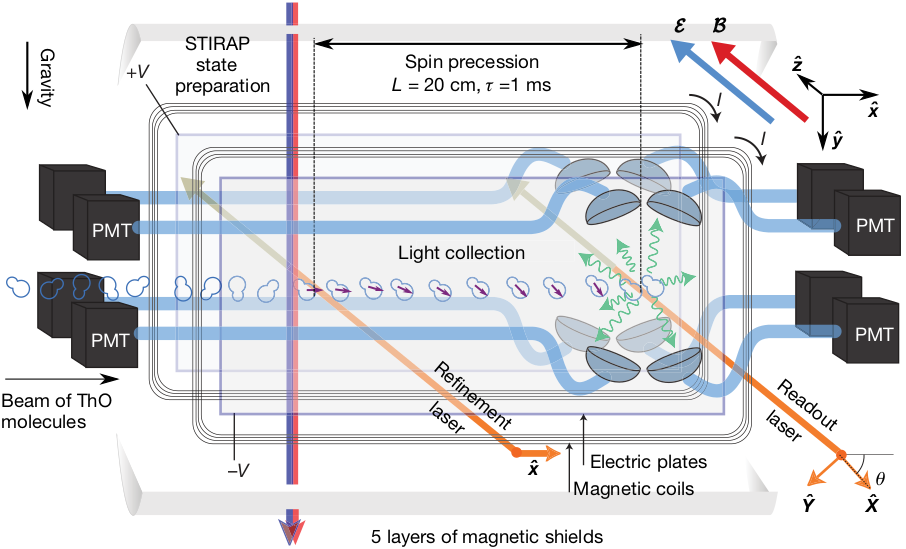
\includegraphics[width = 0.8\textwidth]{Figures/Introduction/eEDM_ACME.png}
                \caption{}
                \label{fig:ACME}
            \end{figure}
        
        \subsubsection{Muon}
            We now come to the muon, to which most of this thesis is dedicated. The $d_\upmu$ search at PSI is going to be discussed in detail in the following chapters but we will here review the current limits. 
            
            \paragraph{Muon \textit{g-2}}
            In 2018 the \textit{g-2} collaboration performed three independent searches for $d_\upmu$.
            All results were compatible with a null value and an upper limit was set: $\abs{d_\upmu}<\SI{1.9e-19}{e\cdot cm}$ \cite{muEDM:direct}.  
            We will here skip the details but we will outline the methods used.\\

            \begin{outline}
                \1[BNL] We saw in \ref{intro:edm} the effect that EDM and MDM have on a moving particle in $\bm{E},\bm{B}$ fields.
                In particular, for muons circulating in a storage ring, the spin precession is given by Eq.~\ref{eq:precession}. 
                The measurement with the $g-2$ detectors is achieved by measuring the oscillation of the vertical component of the positron from the decay. This direction reflects the oscillation of the muon spin.\\
                \1[$g-2$] We will here skip the details but we will outline the methods used. We saw in \ref{intro:edm} the effect that EDM and MDM have on a moving particle in $\bm{E},\bm{B}$ fields. In particular, for muons circulating in a storage ring, the spin precession is given by Eq.~\ref{eq:precession}.\\
                \1[FSD]  We will here skip the details but we will outline the methods used. We saw in \ref{intro:edm} the effect that EDM and MDM have on a moving particle in $\bm{E},\bm{B}$ fields. In particular, for muons circulating in a storage ring, the spin precession is given by Eq.~\ref{eq:precession}.
            \end{outline}
              
            \paragraph{Indirect limit} Given the rise in interest for EDM measurements an effort was undertaken to assess the indirect constraints imposed on $d_\upmu$ by the EDM measurements performed with heavy atoms and molecules~\cite{muEDM:indirect}. 
            This was done by evaluating the $d_\upmu$- induced \textit{Shiff moment}\footnote{As pointed out in \cite{Shiff}, this is the operator inducing the atomic EDM.} of the \ce{^{199}Hg} nucleus, and a specific CP-odd operator for \ce{ThO}.            
            The results, $d_\upmu($\ce{^{199}Hg}$)<\SI{6.4e-20}{e\cdot cm}$ and $d_\upmu($\ce{ThO}$)<\SI{1.9e-20}{e\cdot cm}$, are more stringent than the current measured limit but are \textit{indirect}.
      
\status{review} 
\section{The beams at PSI}
    \label{intro:beamlines}
    
    \status{review}
    \subsection{High-Intensity Proton Accelerator facility}
        \label{sec:hipa}
        The proposal for the accelerator facility at PSI was completed in 1963. The objective was to develop a proton beam of tens of microAmpere and energy above \SI{450}{MeV} to produce $\pi/\mu$.
        The main accelerator is a cyclotron designed to accelerate the beam from \SI{72}{MeV} to \SI{590}{MeV}. 
        The first pre-accelerator, Injector I cyclotron, was developed to accelerate protons and light ions up to \SI{72}{MeV} and \SI{180}{\micro A}
        The performances steadily improved up to \SI{180}{\micro A} but the beam losses at the extraction from the Injector I were the bottleneck.
        The Ring cyclotron was deemed to have the potential to surpass \SI{2}{mA}. For this reason,  in 1978, the proposal of using two pre-accelerators was approved: a \SI{860}{keV} Cockcroft-Walton (CW) followed by a new Injector II cyclotron.\\
        Since 2010 the chain is the following:
        \begin{outline}
            \1 Protons are produced by an electron cyclotron resonance source with a \SI{60}{kV} extraction
            \1 Two solenoids focus the protons onto a collimator: here \ce{^2H+} and \ce{^3H+} ions are stopped
            \1 Protons are then accelerated in three stages
                \2 From \SI{60}{keV} to \SI{870}{keV} by the CW DC linear accelerator, shown in Fig.~\ref{fig:PSI:HIPA:CW}\\
                The beamline connecting the CW to the Injector II is equipped with a bunching system to match the acceptance of Injector II
                \2 Injector II accelerates the pre-bunched beam up to \SI{72}{MeV}
                An electrostatic beam splitter can redirect a fraction of the beam extracted beam (up to \SI{100}{\micro A}) to produce radioisotopes 
                \2 The beam is sent to the Ring cyclotron, shown in Fig.~\ref{fig:PSI:HIPA:cylotron}. Eight magnets keep the particles on the spiral path and four cavities accelerate the beam up to \SI{590}{MeV}
            \1 After the acceleration the beam is extracted and sent to the meson production targets
            \1 The surviving $\sim65\%$ of the beam is sent to the spallation source SINQ (or to a beam dump)
        \end{outline}
            \begin{figure}
            \subfloat[CW feeding the Injector II]{
            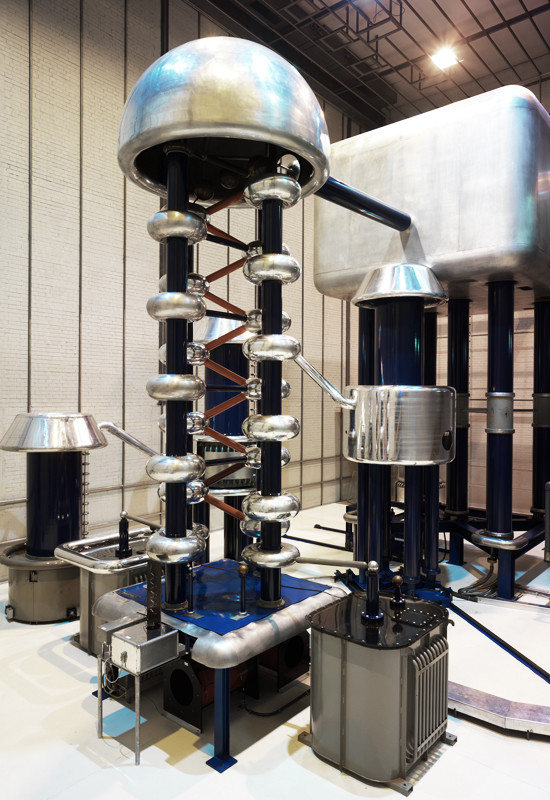
\includegraphics[width=0.47\textwidth, keepaspectratio]{Figures/Introduction/PSI_CW.png}
            \label{fig:PSI:HIPA:CW}}
            \subfloat[Picture of the Ring cyclotron.]{
            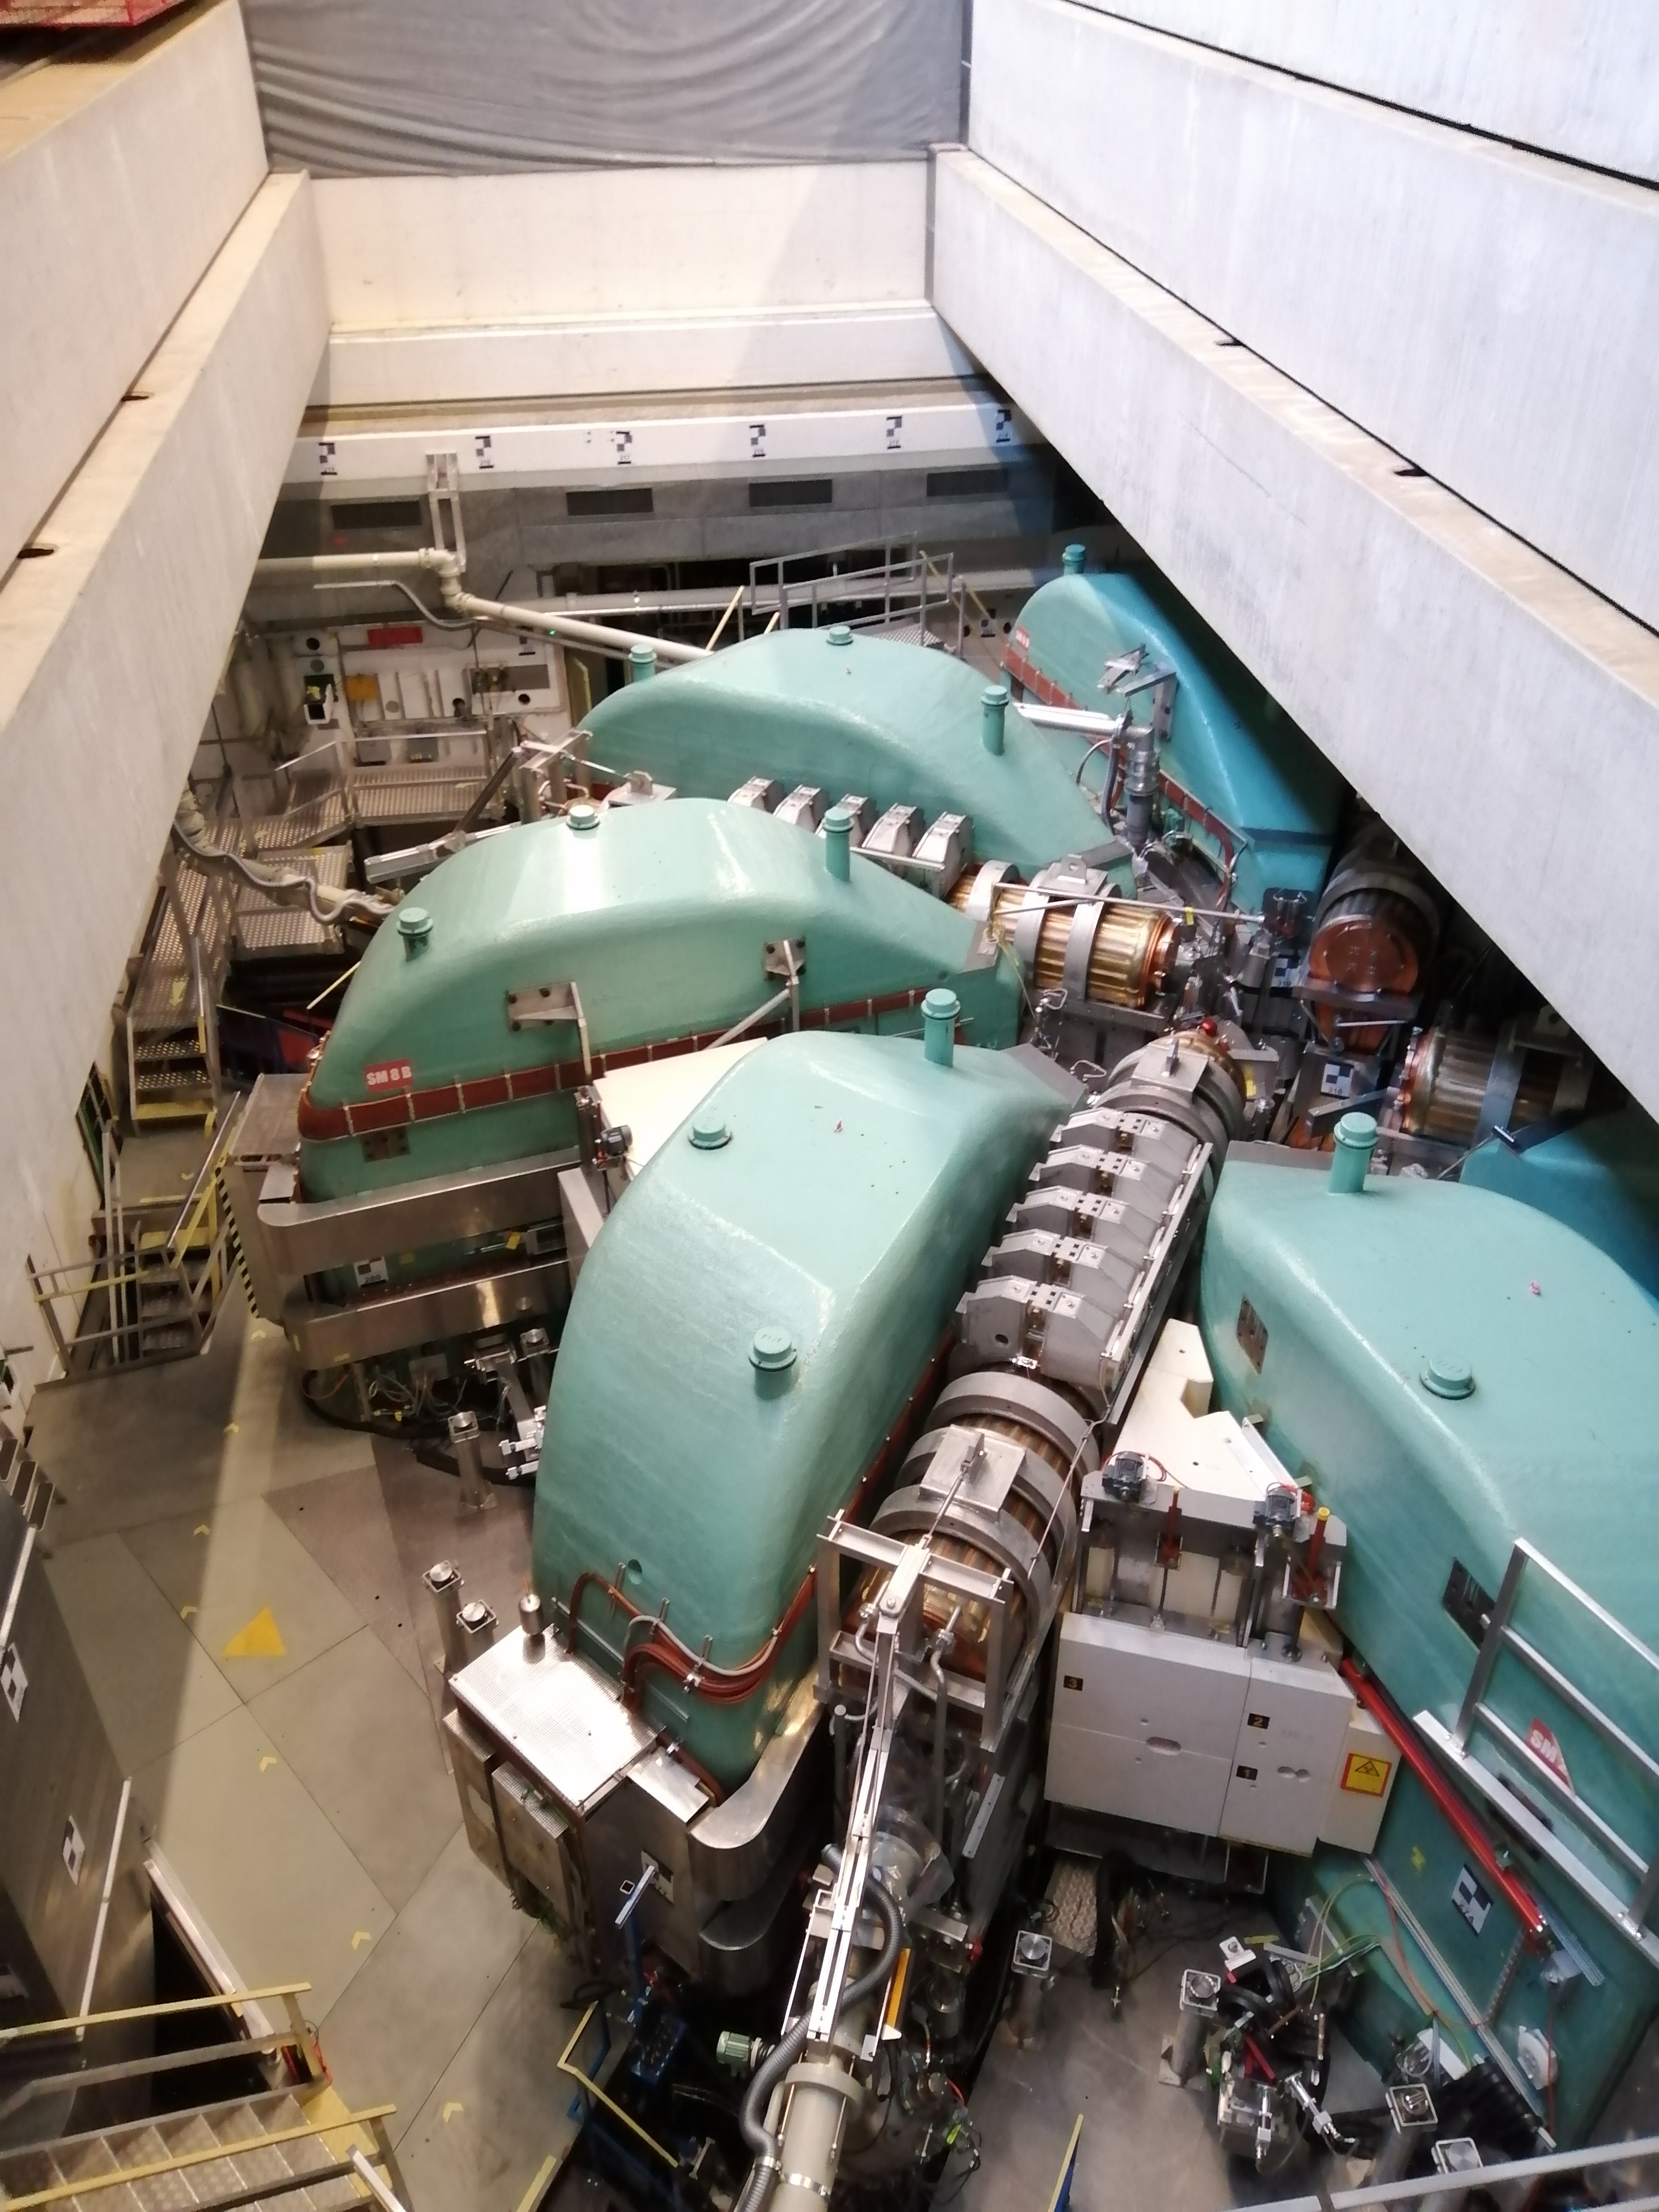
\includegraphics[width=0.51\textwidth, keepaspectratio]{Figures/Introduction/PSI_cyclotron.png}
            \label{fig:PSI:HIPA:cylotron}}
            \caption{Picture of two of the stages of the HIPA facility: the Cockcroft-Walton bringing the proton up to \SI{870}{keV} and the Ring cyclotron accelerating them up to \SI{590}{MeV}.}
        \end{figure}
        \begin{figure}
            \centering
            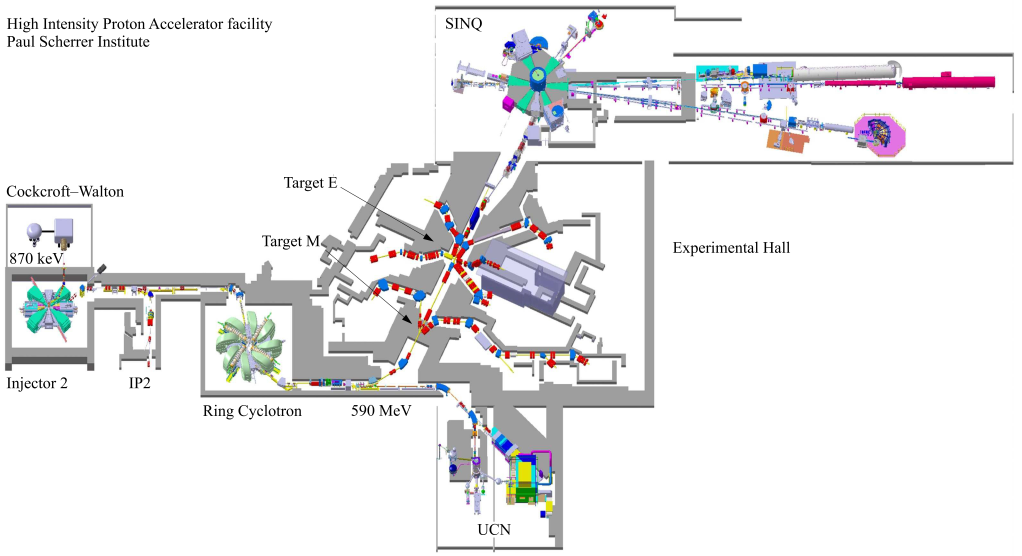
\includegraphics[width = \textwidth]{Figures/Introduction/PSI_HIPA.png}
            \caption{\acrfull{hipa} facility at PSI}
            \label{fig:PSI:HIPA}
        \end{figure}
        
        \paragraph{Injector II}  
        The Injector II cyclotron is designed for high-current operation (\SI{1}{mA} and above) with minimal extraction losses. 
        It achieves high extraction efficiency through a combination of factors: high accelerating voltage, large radius, large gap magnets, and low energy spread. 
        To counter space charge forces, a high vertical betatron tune\footnote{Refers to the number of vertical or horizontal oscillations that a particle undergoes per turn in a cyclotron, indicating the level of vertical or horizontal focusing.} is employed. 
        Injector II is a low-field separate sector machine with four wedge sectors, accommodating two high-voltage double-gap resonators and two single-gap flat-top resonators. 
        Its \SI{870}{keV} injection energy allows for beam collimation and halo cleanup, being below the Coulomb threshold.
        The "vortex motion" is an interesting phenomenon caused by space charge in isochronous cyclotrons \cite{vortexeffect}. 
        For long initial bunches, self-sustaining round sub-bunches are generated, while for short and compact bunches, the vortex effect stabilizes the bunch \cite{vortexeffect:longitudinal} \cite{vortexeffect:transverse}. 
        The PSI operation crew discovered the usefulness of self-focusing, achieving high extracted currents with low losses by operating in an accelerating mode without the need for the flat-top system. 
        In an ongoing upgrade program, Injector II will replace the flat-top resonators with two 50MHz high-voltage resonators. 
        This upgrade aims to reduce extraction losses and enable higher beam currents. 
        Notably, Injector II is the only known production cyclotron worldwide that harnesses the vortex effect.

        \paragraph{Ring cyclotron}
        Over time, the Ring cyclotron's performance was improved, particularly its extraction efficiency. 
        Initially, a well-centered beam was required to pass the Walkinshaw resonance\footnote{The Walkinshaw resonance is a phenomenon in cyclotrons where beams experience a resonance with the machine's magnetic field modulation. Proper alignment and adjustments are necessary to prevent significant beam loss.} without significant loss.
        However, by December 1976, an extraction efficiency of 99.9\% was achieved with a peak intensity of \SI{112}{\micro A}. 
        Ten years later, Injector II alone achieved a beam current of 1mA, and in combination with the Ring cyclotron, reached \SI{310}{\micro A}.
        To increase the intensity, the Ring underwent an RF system upgrade, while a bunching system was implemented in the injection line. 
        The upgrades allowed for a reduction in Ring turns, resulting in a production current of \SI{2.2}{mA} and a beam power of \SI{1.3}{MW}, in line with Joho's $N^3$-Law (see Fig.~\ref{fig:PSI:HIPA:joho}). 
        Further upgrades, including the replacement of the 150MHz flattop cavity, are expected to enable a beam current of \SI{3}{mA} and power of SI{1.8}{MW} for both Injector II and the Ring cyclotron.
        \begin{figure}
            \centering
            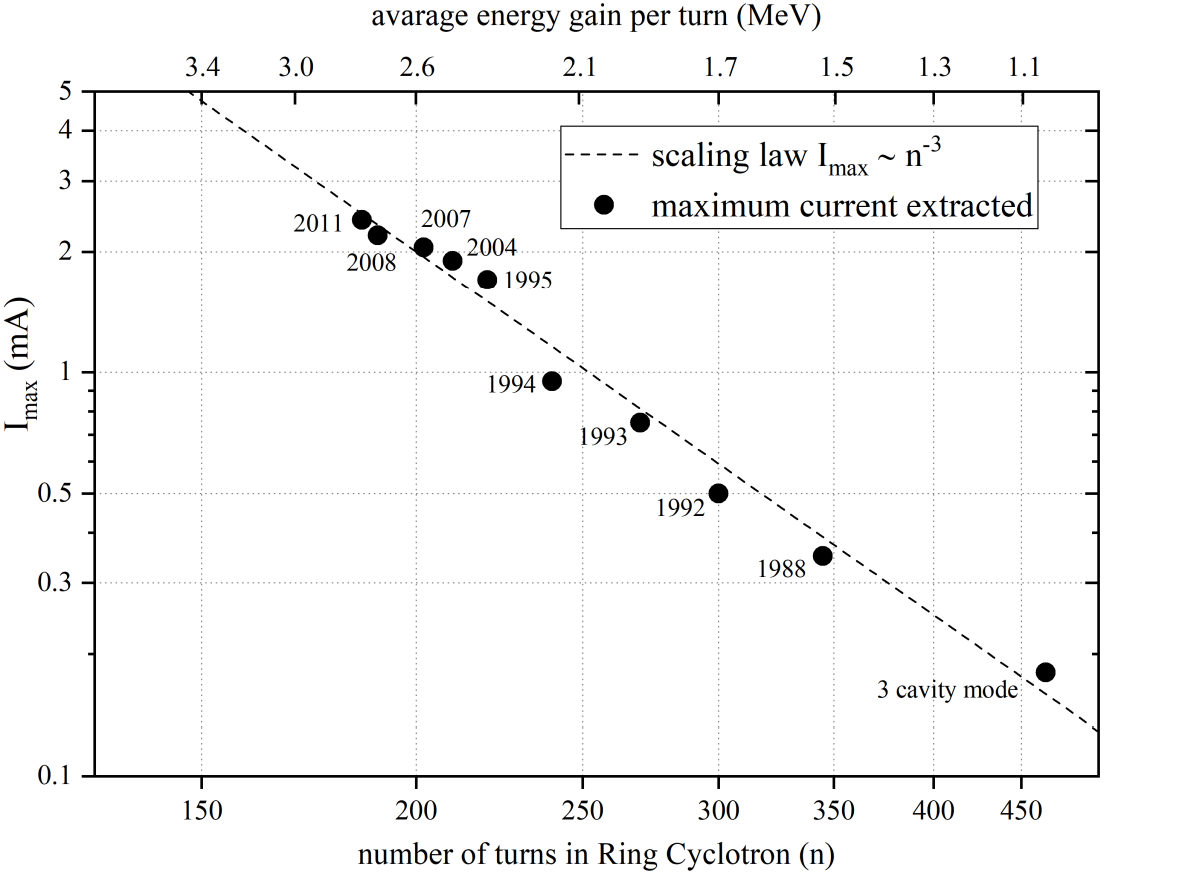
\includegraphics[width = 0.8\textwidth]{Figures/Introduction/PSI_HIPA_joho.png}
            \caption{In 1981, Werner Joho introduced Joho's N3-Law, an analysis of high-intensity issues in cyclotrons \cite{joho}. This law states that the current limit dominated by losses scales inversely with the third power of the number of turns in the cyclotron: $I_{max}\propto N^{-3}$. Remarkably, this formula accurately predicted the performance of the PSI Ring cyclotron for the subsequent two decades.}
            \label{fig:PSI:HIPA:joho}
        \end{figure}
        
        \subsubsection{Performances}
        HIPA operates at a beam power of up to \SI{1.42}{MW}. 
        The maximum beam power (\SI{1.42}{MW}) is limited by the activation and damage of the accelerator components while the maximum beam current authorized is \SI{2.4}{mA}.
        The increase of the beam power in the period between 1974 to 2020 is shown in Fig.~\ref{fig:PSI:HIPA:power}.
        The history of the delivered charge to the meson production targets and SINQ is shown in Fig.~\ref{fig:PSI:HIPA:charge}.  
        A major limiting factor is the scattering of halo particles in the extraction septum.
        There are two key elements for low-loss beam extraction: the generation of beam tails must
        be suppressed as best as possible and the turn separation at the extraction septum must be
        maximized. 
        In this way, the density of halo particles at the position of the extraction septum is minimized.
        The beam is operated 24/7 around 200 days a year. 
        Every three weeks of operation two days of maintenance are scheduled. 
        The details of the different particle production are discussed in the following subsections.

        \paragraph{Power} The experiments at HIPA require high-intensity particle beams for precise measurements, which consume significant electrical power. 
        Upgrades aim to achieve higher particle flux and brightness, necessitating even greater power. 
        Considering the global energy consumption challenges, improving HIPA's energy efficiency is crucial. 
        Fig.~\ref{fig:PSI:HIPA:consumption} displays the power consumption breakdown of the proton facility. 
        During routine operation at a beam current of \SI{2.2}{mA},\SI{1.3}{MW}, the overall power consumption is approximately 12.5MW leading to an efficiency of 11\%.
        For the bare accelerator, the figure is 18\%.
        The RF-to-beam power conversion accounts for the majority of this consumption, around 5.4MW. 
        It scales linearly with beam power, while the power consumption of magnets and auxiliary systems remains independent of the beam power.
        It can be shown that the efficiency can increase with higher current and the aim is >20\% with \SI{3}{mA}
        \begin{figure}
            \centering
            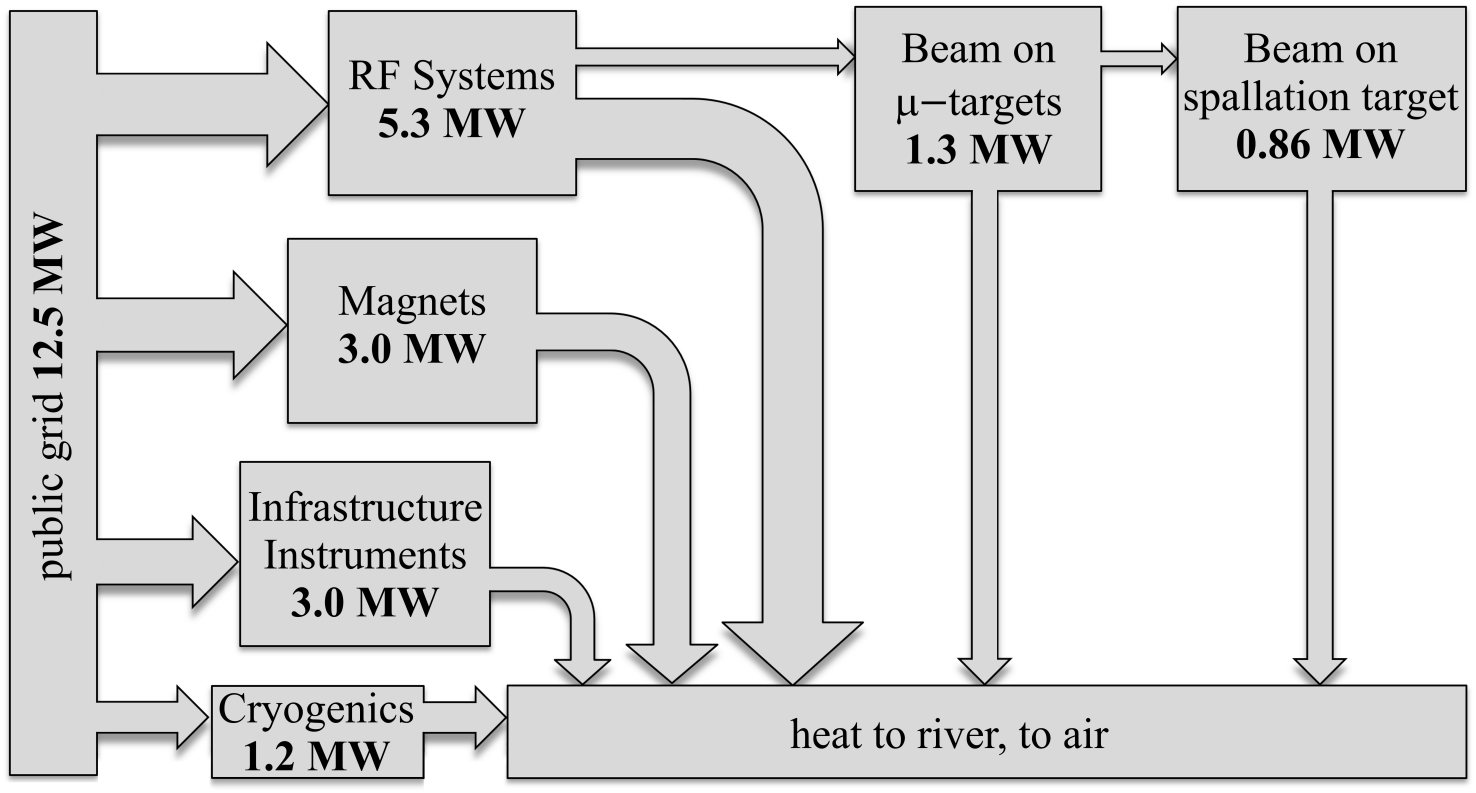
\includegraphics[width = 0.8\textwidth]{Figures/Introduction/PSI_HIPA_consumption.png}
            \caption{Detail of the power usage of the HIPA facility.}
            \label{fig:PSI:HIPA:consumption}
        \end{figure}
        \begin{figure}
            \centering
            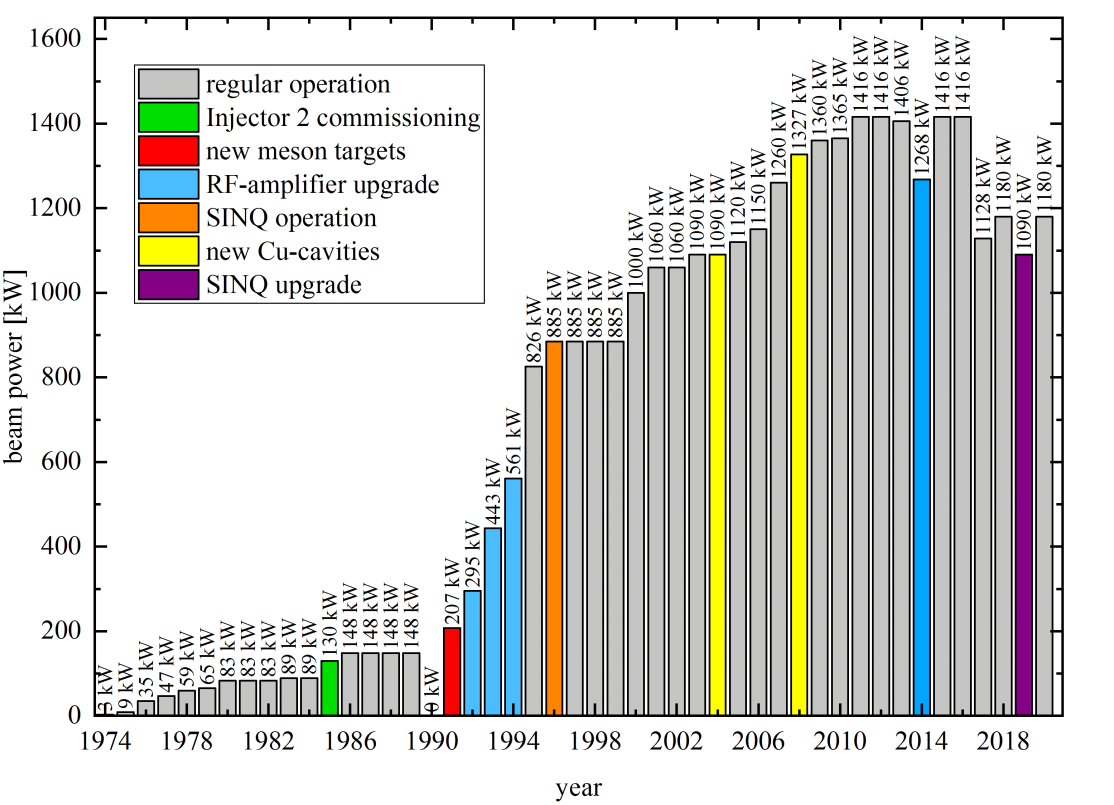
\includegraphics[width = 0.8\textwidth]{Figures/Introduction/PSI_HIPA_power.png}
            \caption{History of the power of the HIPA proton beam.}
            \label{fig:PSI:HIPA:power}
        \end{figure}
        \begin{figure}
            \centering
            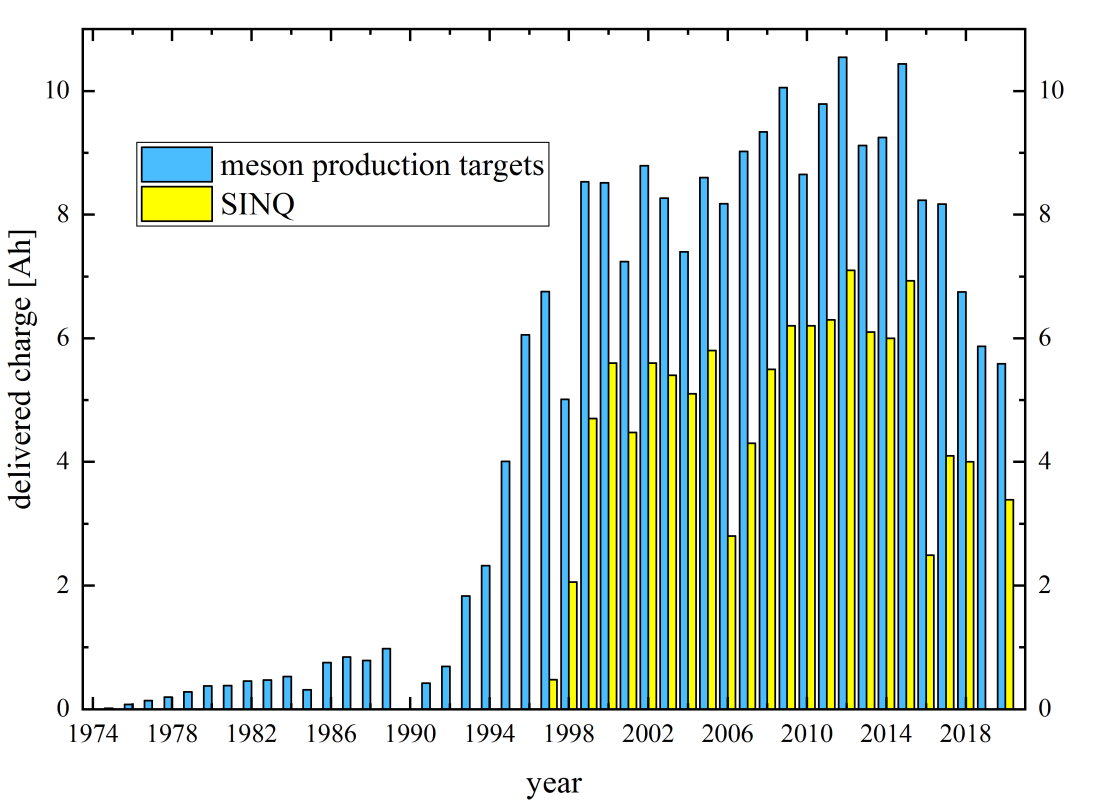
\includegraphics[width = 0.8\textwidth]{Figures/Introduction/PSI_HIPA_charge.png}
            \caption{History of the charge delivered by the HIPA beam on the meson production targets and SINQ.}
            \label{fig:PSI:HIPA:charge}
        \end{figure}
   
    \status{review}
    \subsection{Meson production}       
        \label{sec:hipa:M}
        As we saw in \ref{sec:hipa}, \gls{hipa} delivers a continuous $2.4$ mA $590$ MeV proton beam. 
        To have a high pion/muon yield a low Z material is the best choice for the Meson Production Targets: graphite is has been used since 1990's.
        The whole system (target, collimators, beam dumps, \dots) has to be cooled and, due to nuclear reactions, is highly radioactive.
        Pions are produced by the interaction with nucleons in the target (threshold at 280 MeV in the center-of-mass frame) and muons are then produced by pion decay.
        When $\pi$ are stopped at $\sim 1$ mm from the surface of the target, $\mu^+$ can escape and are called \textit{surface muons}.
        These muons have energies below 4.1 MeV ($p=29.8$ MeV) and are $\approx100\%$ polarized.
        Muons created by in-flight decay have higher energies and are cooled \textit{cloud muons}. Both positive and negative muons are possible but the negative charge is suppressed by a factor $\sim 3$.
        There are two targets: M feeds two beamlimes (PiM1 and PiM3; E feeds 5 beamlines (PiE1, MuE1, MuE4, PiE3, PiE5).
        The detail of the facilites are summarized in Tab.~\ref{tab:PSI:beamlines}
        The targets are graphite wheels which rotate to distribute the heat due to the impinging beam.
        The material is polycrystalline graphite made of small crystallites of $\sim2$\SI{0}{\micro m} irregularly arranged.
        \begin{table}[]
            \centering
            \begin{tabular}{|c|c|c|c|c|}
                 \hline
                 Target & User facility & Particles & Momenta (MeV/c) & Rate ($s^{-1}mA^{-1}$)\\
                 \hline
                 \hline
                 \multirow{ 2}{*}{M (\SI{5}{mm})} 
                 & $\pi$M1 & e/$\uppi/\upmu/$p & 10-450 & \SI{2e8}{} \\
                 & $\pi$M3.1-3 & $\upmu/$ & 10-40 & \SI{3e6}{}\\
                 \hline
                 \multirow{ 5}{*}{E (\SI{4/6}{cm})} 
                 & $\pi$E1 & $\uppi/\upmu/$p & 10-450 & \SI{1e9}{}\\
                 & $\pi$E3 & $\upmu$ & 10-40 & \SI{3e7}{}\\
                 & $\pi$E5 & $\uppi/\upmu$ & 10-120 & \SI{5e8}{}\\
                 & $\pi$E1 & $\upmu$ & 60-120 & \SI{6e7}{}\\
                 & $\pi$E4 & $\upmu$ & 10-40 & \SI{4e8}{}\\ 
                 \hline
            \end{tabular}
            \caption{Particle types available at the meson facilities. The rate in particles per second per \SI{1}{mA} of proton}
            \label{tab:PSI:beamlines}
        \end{table}
        
        \paragraph{E Target}
        The target is inserted vertically into the beamline and held by a horizontal rotating shaft. The graphite and the hub are connected by six spokes. 
        While operated at \SI{2}{mA}, the temperature of this \SI{40}{mm}/\SI{60}{mm} target is \SI{\sim1700}{K}. Water-cooled copper shields are mounted on the rear of the target. To reduce the deformations the graphite rim is made of 12 segments. 
        Variations of the beam positions are crucial and to improve the sensitivity the graphite wheel was modified: small grooves were applied on both sides. This modulates the beam transmission.
        At the end of 2019 a new target wheel was tested, having a small angle for the impinging beam. 
        This \textit{slanted target} keeps the effective thickness creating a larger active surface and two different spots for IN/OUT of the beam. The net effect is an increase $\sim50\%$ in the surface muons.
        As the bearings degrade from heat and radiation they have to be replaced after a few months of operation. The procedure for the maintenance of the target here will not be discussed.
        
        \paragraph{M Target}
        This target is smaller in thickness and the bearings are far from the beam thus the demands are less challenging. 
        The rim of the target is \SI{2}{cm} wide and \SI{2}{mm} thick.  
        With an impinging angle of \SI{30}{\deg} the effective thickness is \SI{5.2}{mm} inducing a beam loss of $1.6\%$. 
        The target operates at \SI{1100}{K} and is cooled by conduction.
        For the upcoming \gls{himb} the aim is to increase the muon rate by a factor up to 100. 
        For this purpose studies for an upgrade of the M target station, with a slanted target design, are ongoing.
        A similar slanted target was already tested in the E target station, yielding a $\sim 50\%$ increase in surface muon rate.
        
        \paragraph{Collimators and Beam dump}
        Just like target E, Collimators and beam dump are inserted vertically and shielded.
        Both are made of oxygen-free copper: improve thermal conductivity; avoid hydrogen embrittlement \footnote{Hydrogen can be produced by the spallation reaction of the protons with copper. This hydrogen can bond with oxygen creating water molecules that can produce cracks in the copper.}; for brazing of the steel tubes onto the copper body.
        To avoid any significant change in the material, the copper is kept below \SI{400}{K} using water-cooling.
        The collimator system as well as the beam dump have to stand more than 100 kW per component.
        The water flows in stainless steel pipes are wound outside and brazed on the cylindrical body. 
        This is done to avoid direct contact of the proton beam with the water, which would create corrosion-inducing ions.
        The main body is made of six slices brazed together.
        The shape and manufacture of these sections were optimized using computational fluid dynamics in order to reduce the energy deposit and thermal stress.
        An aperture, made of 4 slits of \SI{100}{\mu m} Nikel foils, is mounted in front of the devices.
        Here free electrons from ionization are collected and used for beam position and size monitoring.
        Aside from a water leak problem, likely due to thermal stress, no visible signs of radiation damage are observed since installation.
        
    \status{review}
    \subsection{Neutron production}
        \subsubsection{SINQ}
            The first spallation neutron source built at PSI was SINQ, which has dedicated neutron scattering instruments and was used as a polarized cold-neutron beam line for fundamental neutron physics.
            After passing through the meson production target the proton energy is degraded to \SI{570/565}{MeV}. 
            The beam is bent downwards and then up vertically onto the spallation target.
            The thermal neutron flux scales with the beam current and is $\sim$\SI{1.5e14}{cm^{-2}s^{-1}} near the target.
            This beamline was used for many measurements conducted in preparation for the UCN source and many parameters of UCN production (and loss) were here determined.
            
        \subsubsection{UltraCold Neutrons}
            Neutrons below \SI{4}{mK} are called UltraCold. 
            This corresponds to energy below \SI{300}{neV}, which is comparable with the gravitational potential of a neutron at a few meters height and also the neutron optical potential: material bottles can hence contain UCNs.        
            The design of the UCN source, shown in Fig.~\ref{fig:UCN_CAD}, was presented in 2000 to push the sensitivity of the nEDM search.
        
            \paragraph{Source setup}
            The HIPA \SI{590}{MeV} proton beam is deflected by a magnetic kicker and sent in the spallation source.
            Each spallation reaction with the lead atoms leads to an average of 8 neutrons, which are then thermalized in heavy water.
            The main moderator is made of solid deuterium at \SI{5}{K}.
            The UCN produced exit the moderator's vessel through a thin aluminum lid in a vertical guide and their energy is lost to gravity.
            From here the UCN are delivered via  long neutron guides: two at the bottom and one at the top of the vessel.
            The 30 liters of solid D$_2$ is the core of the whole system and takes several days to achieve a good ice quality.
            UCN intensity reflects the quality of the achieved solid deuterium, as shown in Fig.~\ref{fig:UCN_behaviour} exemplifying a typical UCN intensity behavior during such a slow freezing process.
        
            \paragraph{Performance}
            A key parameter in the performance of a UCN source is the number of particles delivered.
            The exponential decay measured at the lower ports reflects the emptying time of the central storage vessel.
            Measuring in the higher port a faster exponential is found, demonstrating that the UCNs with energies high enough to reach that port are quickly drained.
            Several studies to understand all aspects of the UCN source have been conducted since its inauguration, as well as the UCN transport from production in the solid deuterium to a beam port.
            A slow decrease in performance was discovered and a temperature-cycling ``conditioning'' was developed to regain maximum UCN intensity.
            The UCN source has been reliably operating since 2011 (see Fig.~\ref{fig:UCN_stats}).
    
            \paragraph{Results}
            The resulting nEDM limit $d_n = (0.0 \pm 1.1_{stat}\pm0.2_{sys})\times$\SI{e-26}{e cm} was published in 2020 \cite{nEDM} but other results were also obtained thanks to this facility:
            \begin{itemize}
                \item A measurement of the mercury-to-neutron magnetic moment ratio
                \item Spin-echo spectroscopy with ultracold neutrons
                \item Measurement of gravitational depolarization of ultracold neutrons
                \item limit for oscillating electric dipole moments
                \item limit for spin-dependent forces mediated by axion-like particles
            \end{itemize}
            \begin{figure}
                \centering
                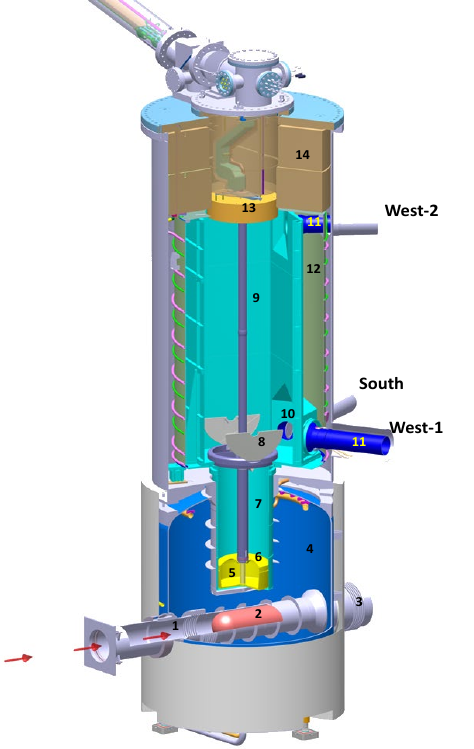
\includegraphics[scale = 0.5]{Figures/Introduction/UCN_CAD.png}
                \caption{CAD for the UCN source taken from  \cite{PSI:review:2021}. Some of the key aspects are: 2 - lead spallation source, 4 - heavy water moderator, 5 - D$_2$ moderator, 9 - storage vessel, 10 - 11 UCN guide and guide shutter.}
                \label{fig:UCN_CAD}
            \end{figure}
            \begin{figure}
                \centering
                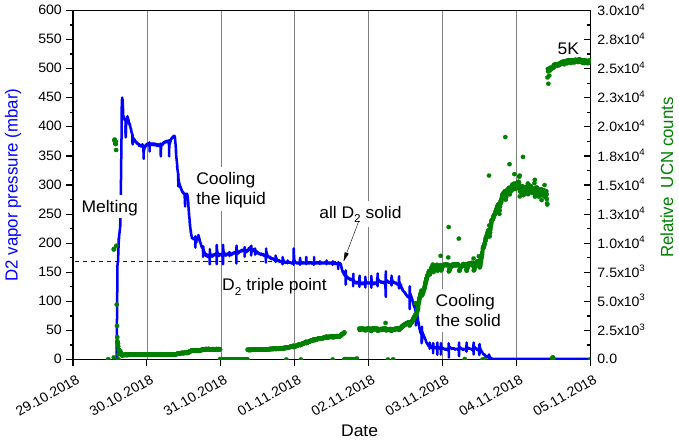
\includegraphics[width = 0.8\textwidth]{Figures/Introduction/UCN_behaviour.png}
                \caption{The observed behavior during the slow freezing of the deuterium. The large increase in UCN output demonstrates the strong reduction in UCN losses within the D$_2$. 
                Figure taken from \cite{PSI:review:2021}}
                \label{fig:UCN_behaviour}
            \end{figure}
            \begin{figure}
                \centering
                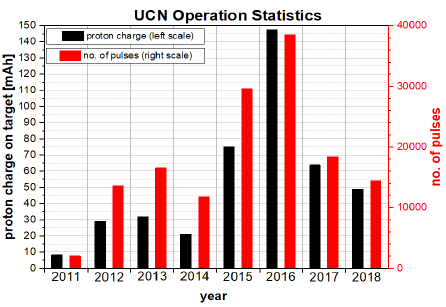
\includegraphics[width = 0.8\textwidth]{Figures/Introduction/UCN_stats.png}
                \caption{Annual statistics of the UCN source showing total accumulated beam current on target (black bars) and number of beam pulses (red bars) on the UCN spallation target. 
                Figure taken from \cite{PSI:review:2021}}
                \label{fig:UCN_stats}
            \end{figure}
            
    \status{review}
    \subsection{High-Intensity Muon Beams}
        Currently, PSI delivers the most intense continuous muon beam in the world with up to a few \SI{e8}{\upmu^+/s}.
        The High-Intensity Muon Beams (HiMB) project at PSI focuses on the development of a new target station and muon beamlines to deliver up to \SI{e10}{\upmu^+/s} \cite{HIMB:2021}\cite{HIMB:gio}.
        The aim is to boost the production, collection, and transport of surface muons.
        HIMB is part of the  Isotope and Muon Production using Advanced Cyclotron and Target Technologies project (IMPACT)\cite{impact}.

        \subsubsection{Production and collection}
        To increase the surface muon yield, the M target discussed in \ref{sec:hipa:M} will be substituted with target H, having a more slanted geometry.
        This new target, shown in Fig.~\ref{fig:himb:target}, will be \SI{20}{mm} thick in the proton direction, with a \SI{10}{deg} slanting angle: surface muon yields comparable to a 40 mm thick non-slanted target. 
        The protons will impinge below the rotation shaft (Fig.~\ref{fig:himb:target:b}), from the back of the target, in a copper water-cooled shielding (Fig.~\ref{fig:himb:target:a}).
        The target will fit in the remote-controlled exchange flask of target E for easier handling and maintenance.
        \begin{figure}
            \centering
            \subfloat[Section of the HIMB H target.]{
            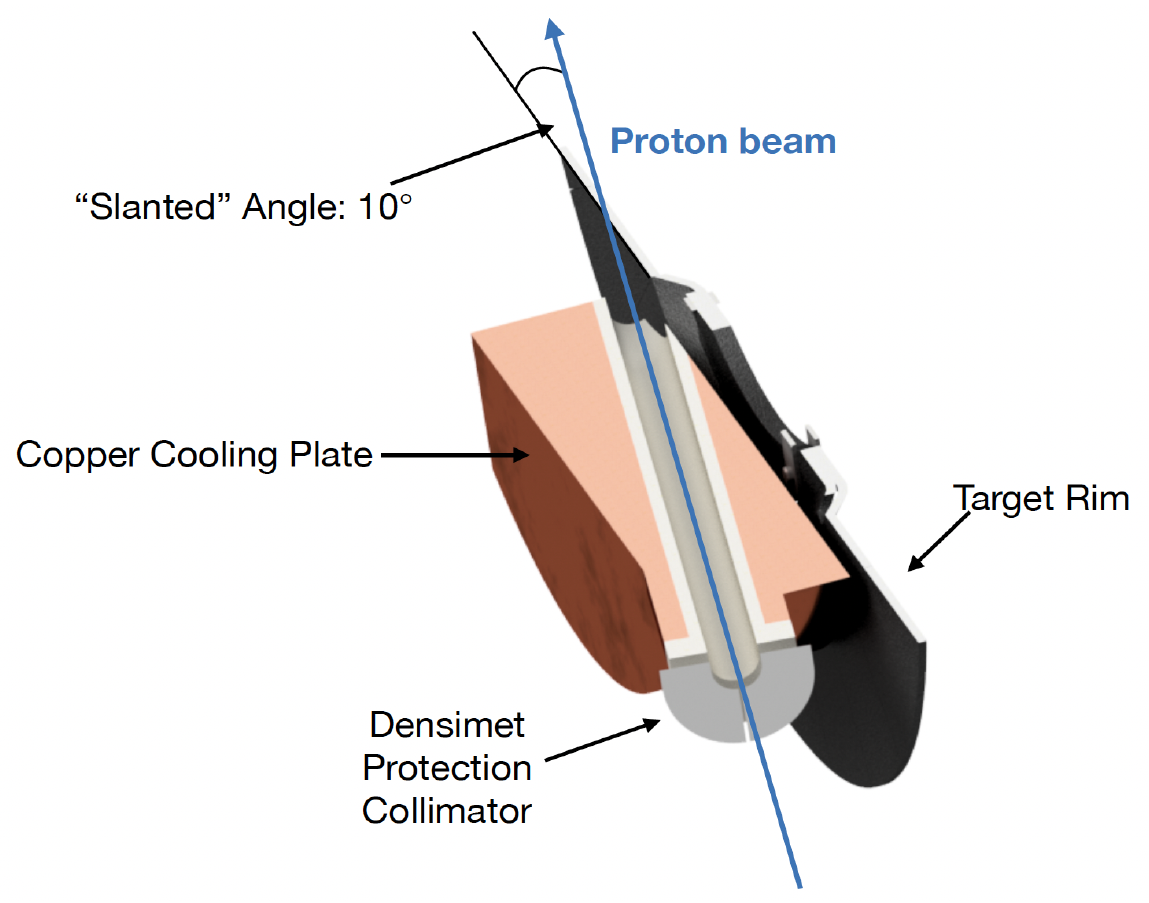
\includegraphics[height=4.5cm, keepaspectratio]{Figures/Introduction/himb_target_section.png}
            \label{fig:himb:target:a}}
            \subfloat[Side views of the HIMB H target]{
            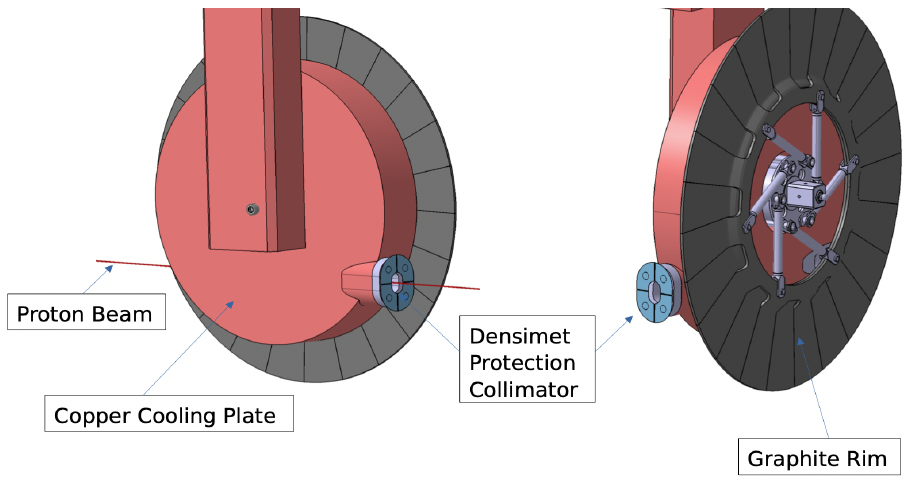
\includegraphics[height=4.5cm, keepaspectratio]{Figures/Introduction/himb_target.png}
            \label{fig:himb:target:b}}
            \caption[HIMB H target]{Depiction of the target H for the HIMB project. The slanted target improves the production of surface muons. \textbf{a)} The proton beam impinges from the back side passing through a copper water-cooled shielding. \textbf{b)} The beam travels lower to avoid the rotating shaft.}
            \label{fig:himb:target}
        \end{figure}
        
        \noindent
        When using solenoids to capture particles, the target is often completely enclosed in the solenoid aperture. 
        This solution is not viable for HIMB because the proton beam is not stopped in the H target. 
        The proposed solution, shown in Fig.~\ref{fig:himb:solenoids}, is to have two different NC solenoids (\SI{\sim 0.45}{T}) sideways to the target. 

        \begin{figure}[h]
            \centering
            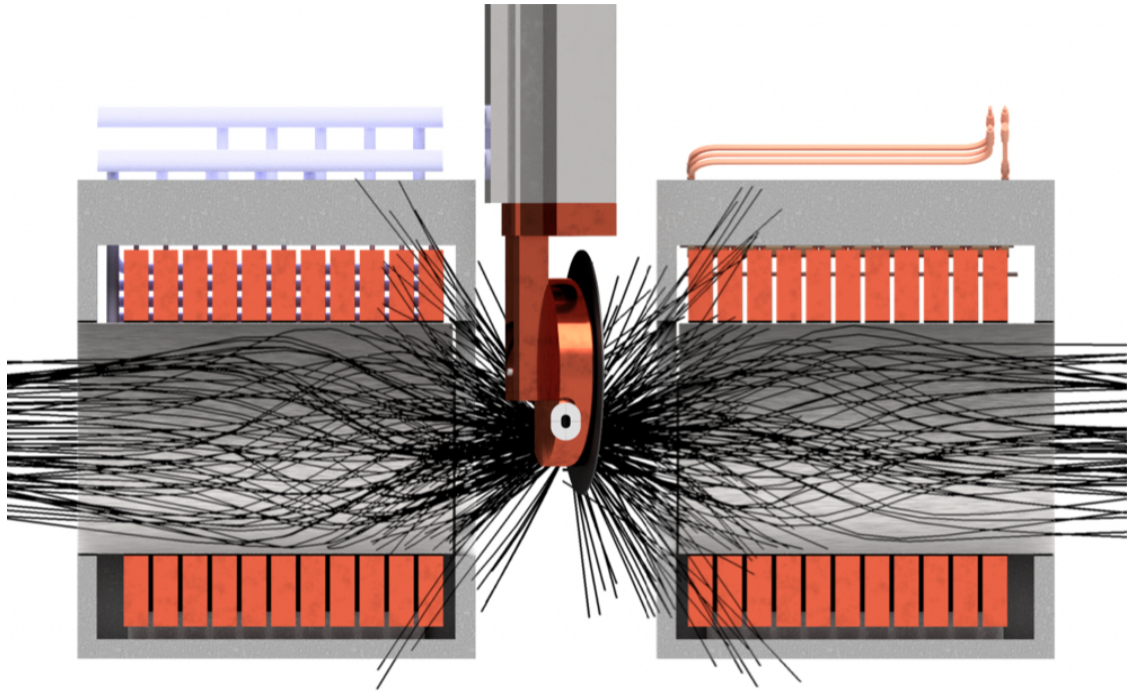
\includegraphics[width=0.8\textwidth]{Figures/Introduction/himb_solenoids.png}
            \caption[HIMB solenoids]{HIMB will have two different NC solenoids sideways to the target. These are required to collect the produced muons and let the surviving proton beam continue toward the spallation SINQ setup.}
            \label{fig:himb:solenoids}
        \end{figure}

        \noindent
        The particles produce by the impact of the \SI{590}{MeV} proton beam are: electrons, muons and pions.
        The momentum spectrum of the generated particle is shown in Fig.~\ref{fig:himb:momenta}: the peak in the $\upmu^+$ spectrum is caused by surface muon production while, at higher energies, the muons come from pion decay in flight. 
        This peak is not present for $\upmu^-$ because stopped $\uppi^-$ undergoes nuclear capture and no muons are produced.  
        In a similar fashion, the peak in positron around Michel edge is produced by stopped $\upmu^+$.
        The HIMB project focuses on surface muons but the optimization are done to accept and transport momenta up to \SI{80}{MeV/c}, while keeping the focus on \SI{28}{MeV/c}.
        
        \begin{figure}[h]
            \centering
            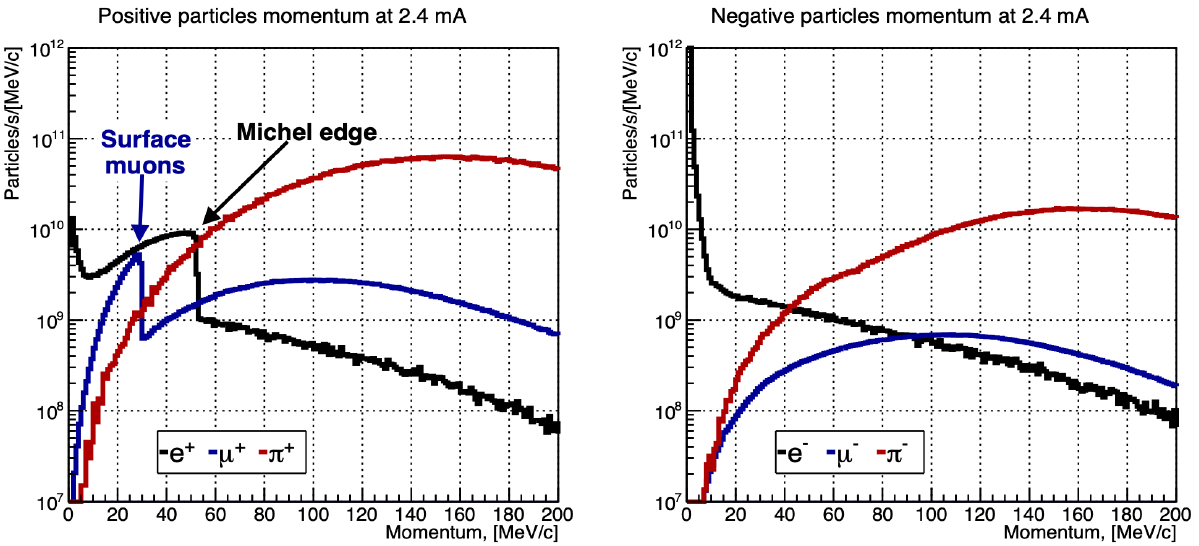
\includegraphics[width=0.9\textwidth]{Figures/Introduction/himb_momenta.png}
            \caption[HIMB momentum spectrum]{Momentum spectrum for positive and negative $e,\upmu,\uppi$ produced at the HIMB H target for a proton current of \SI{2.4}{mA}.}
            \label{fig:himb:momenta}
        \end{figure}
        
        \subsubsection{Beamlines}
        HIMB will introduce two beamlines: MUH2 and MUH3.
        The peculiarity of these lines is the extensive use of solenoids.
        Solenoids achieve focus on both axes (wrt. quadrupoles) but usually, their usage is limited by the required magnetic fields. 
        For the momentum of the surface muons \SI{\sim 0.45}{T} are sufficient and achievable with NC solenoids. 
        
        The MUH2 beamline is designed to deliver beams to fixed target experiments (e.g. Mu3e). It will be located at the left-hand side of the target station and its most important figure of merit for MUH2 is transmission.
        Two 40 deg bends are included in the beam trajectory with dipoles to avoid a direct line of sight to the target.\\
        The model reported in the Conceptual Design Report (CDR) published in January 2022 [10] is able to deliver \SI{1.22e10}{\upmu^+/s} at a proton current of \SI{2.4}{mA} at the entrance of the experimental area at the surface muon momentum. 
        The beam spot size and the average polarization at the end of the channel are $\sigma_x = 40$ mm, $\sigma_y = 42$ mm, and $\varepsilon = 0.88$.
        Interesting to note that a double Wien filter scheme is currently under study to keep the positron contamination under control.
 
        The MUH3 beamline, on the right-hand side of the target station, aims at delivering muon beams for muon spin rotation spectroscopy ($\upmu$SR).
        For these applications, \SI{e10}{\upmu/s} is not required and part of the beamline follows a more standard approach with quadrupoles.
        From simulations, while the solenoid section delivers more than \SI{e10}{\upmu/s}, the rate drops to \SI{3e8}{\upmu/s} at \SI{15}{MeV} and \SI{6e6}{\upmu/s} at \SI{10}{MeV} when reaching the two experimental area.
        The expected beam spots and polarization are $\sigma_x = 40$ mm, $\sigma_y = 42$ mm, and $\varepsilon\gtrsim 0.95$.
        
\status{review}
\section{Proton Ionization Facility}
    Another interesting facility at PSI is the Proton Ionization Facility (PIF) \cite{PIF:1996}\cite{PIF:2001}.
    This was designed, in conjunction with the European Space Agency, to be a user-friendly testing ground for spacecraft components.
    The deteriorating effect that high-energy protons can have on semiconductors is a key aspect of the correct functioning of spacecraft in the space environment.
    Depending on the orbit and the duration of the flight the exposure to this hazard can vary and having reproducible test grounds is cardinal during the design phase. 
    The original goals of this facility:
    \begin{outline}
        \1 Radiation hardness of the new electronic products
        \1 Single Event Upsets (SEU) and Latch-ups (SEL) of electronic components
        \1 Properties of radiation monitors for space and laboratory applications
        \1 Basic mechanics of radiation effects in semiconductors
        \1 Space radiation environment by on-earth simulations
    \end{outline}
    Given the broad range of energy and intensities of the facility, alongside ESA many other users apply for beamtime at PIF within the accelerator communities, such as CERN, but also external laboratories, industries, and universities.
    During the daytime, the beam is usually reserved for biomedical applications and these irradiation studies are done parasitically during the night and on weekends.
    Although only for a short period, I joined PIF and I had the opportunity to be a shifter. 
    It was quite an interesting experience, allowing me to become acquainted with a different setup and to see a different aspect of the research in particle physics.
    The usual shift would consist in tuning the beam to be suited to the user's needs and supporting during the data taking.

\status{started}
\printbibliography[
    heading = bibliographychapter,
    title=Bibliography for the introduction
]

\end{refsection}